\chapter{Results}\label{chapter:Results}
%TODO: move all information from Pros/cons in text and remove column from table!


The experiments involved in this chapter can be organised in two parts: First, a preliminary analysis on the differences between distinct model variants is presented. More specifically, different options for the past frame encoder, the matching strategy and the decoder are compared. Additionally, an expanded multi-scale version of the mask encoder with the option to include multiple descriptors per predicted class is involved in the comparisons. \par

Model variants are compared in terms of their performance on our test set as well as the cross domain evaluation set DAVIS. Apart from performance criteria, the inference time and GPU allocation are included in the method comparisons to indicate differences in the computational cost of each option. \par 

In the second part of the analysis, the best performing variant of the proposed method is compared to a naive heuristic-based tracking baseline built on the unknown instance segmentation method INSTR and the semi-supervised tracking method HODOR. At the end of the chapter, a qualitative assessment of our proposed method with INSTR on recorded real-world data initialisation is presented.

\section{Preliminary experiments} \label{seq:preliminary_exps}


\subsection{Encoder comparisons}

The first type of performed model comparisons is between different types of past frame encoders. Specifically, the backbone image encoder, the bounding box encoder and the mask encoder are compared. The mask encoder is included in the analysis in two versions, with and without layernorm computation before matching, with the first option resembling more the masking strategy of HODOR \parencite{athar2022hodor}. \par
All experiments are performed with the same attention-based matching mechanism and FPN decoder for a more fair comparison. The four encoder variants are compared in terms of their performance both on the synthetic tracking test set and the DAVIS evaluation set. It is worth noting that the DAVIS evaluation set consists of real images and provides an indication on the \gls{sim2real} performance gap for models trained on synthetic data, that are meant to be deployed in real life scenarios. All methods are evaluated with regard to their performance on both datasets based on the achieved $J, F,$ and$ J\&F$ scores. For the tracking dataset, also the inference time is included in the evaluation \tabref\ref{Tab:encoder_comparisons}. \par
% as an indication of the computational cost each variant poses to the GPU. An overview of the obtained results is provided in Table 

\begin{table} [ht!]
\caption{Comparison of encoder types}
\centering
\begin{tabular}{|c|ccc|ccc|c|}
\hline
\multicolumn{1}{|c|}{\multirow{2}{*}{Encoder Type}} & \multicolumn{3}{c|}{Tracking Dataset}                                              & \multicolumn{3}{c|}{Davis} & \multicolumn{1}{c|}{\multirow{2}{*}{time [s]}}                                                         \\ \cline{2-7} 
\multicolumn{1}{|c|}{}                              & \multicolumn{1}{c|}{J} & \multicolumn{1}{c|}{F} & \multicolumn{1}{c|}{J\&F} & \multicolumn{1}{c|}{J} & \multicolumn{1}{c|}{F} & \multicolumn{1}{c|}{J\&F}  & \multicolumn{1}{c|}{}                             \\ \hline

backbone    &   0.691  &  0.780  &  0.735 &   0.443   &  0.539   &    0.491  & 0.0986   \\ 

bbox &  0.600 &   0.703   &   0.651    &   0.361     &   0.442      &  0.406  &  0.0711 \\ 

mask without mean  &   0.718 &   0.808   &   0.763   &  0.430  & 0.507  & 0.469   & 0.0704 \\ 

mask with mean  &  0.708 &   0.797  & 0.752    & 0.438 & 0.524  & 0.481  & 0.0714  \\ \hline

\end{tabular}
 \label{Tab:encoder_comparisons}
\end{table}




\begin{figure} [ht!]
    \centering
    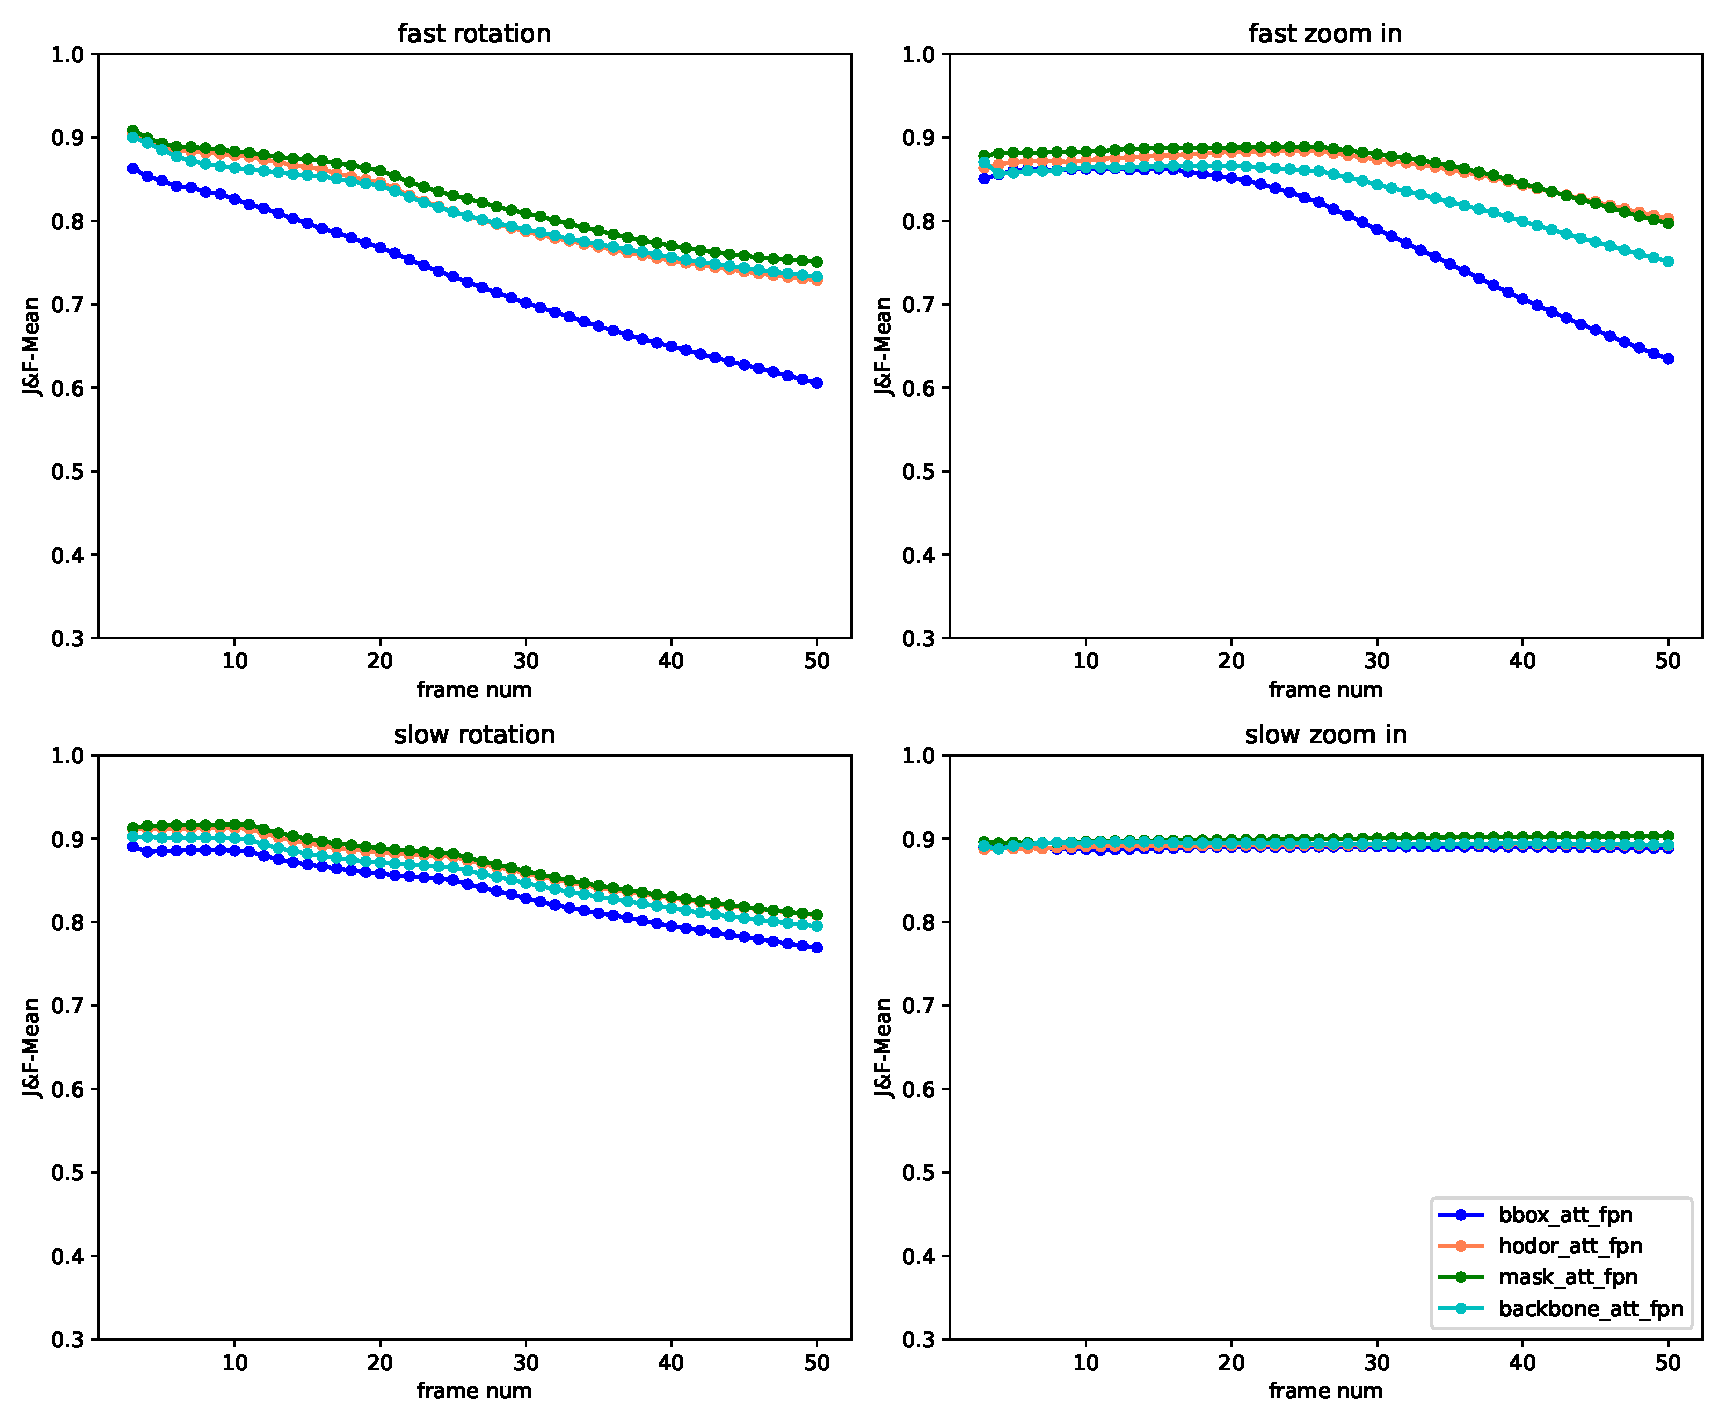
\includegraphics[width=1.\linewidth]{figures/04_experiments/encoder_ablations/bbox_att_fpn-hodor_att_fpn-mask_att_fpn-backbone_att_fpn-movement_all.pdf}
    \caption{Temporal analysis of encoder variants}
    \label{fig:all_encoders}
    
\end{figure}

Comparing the four variants in terms of their performance on the synthetic tracking dataset, the mask encoder without LayerNorm (denoted as 'without mean' in \tabref\ref{Tab:encoder_comparisons} before matching appears to achieve the highest $J\&F$ score. The backbone encoder also achieves comparable average performance, but requires longer inference time, since two twin SegFormer-B3 backbones are involved in the forward function. Finally, as expected, the bounding box encoder achieves the poorest performance, since the past propagated information is merely a motion cue, 
%acting similar to positional encodings, 
instead of a rich past feature representation. \par


For a more detailed comparison of different encoder types, a temporal analysis was performed, where the cumulative $J\&F$ mean was computed for 50 frames on each scene. The test set scenes were divided into groups based on the type of camera motion encountered in the scene (rotational/zoom in) and the camera velocity (fast/slow). This grouping of the available scenes aims at better highlighting the differences in performance achieved by different encoding strategies depending on the scene difficulty, which is related to the camera movement type. Additionally, for a better indication of the range of performance scores between different scenes within each group, the variance is included in the plots, see \figref\ref{fig:all_encoders_var}.\par



\begin{figure} [ht!]
    \centering
    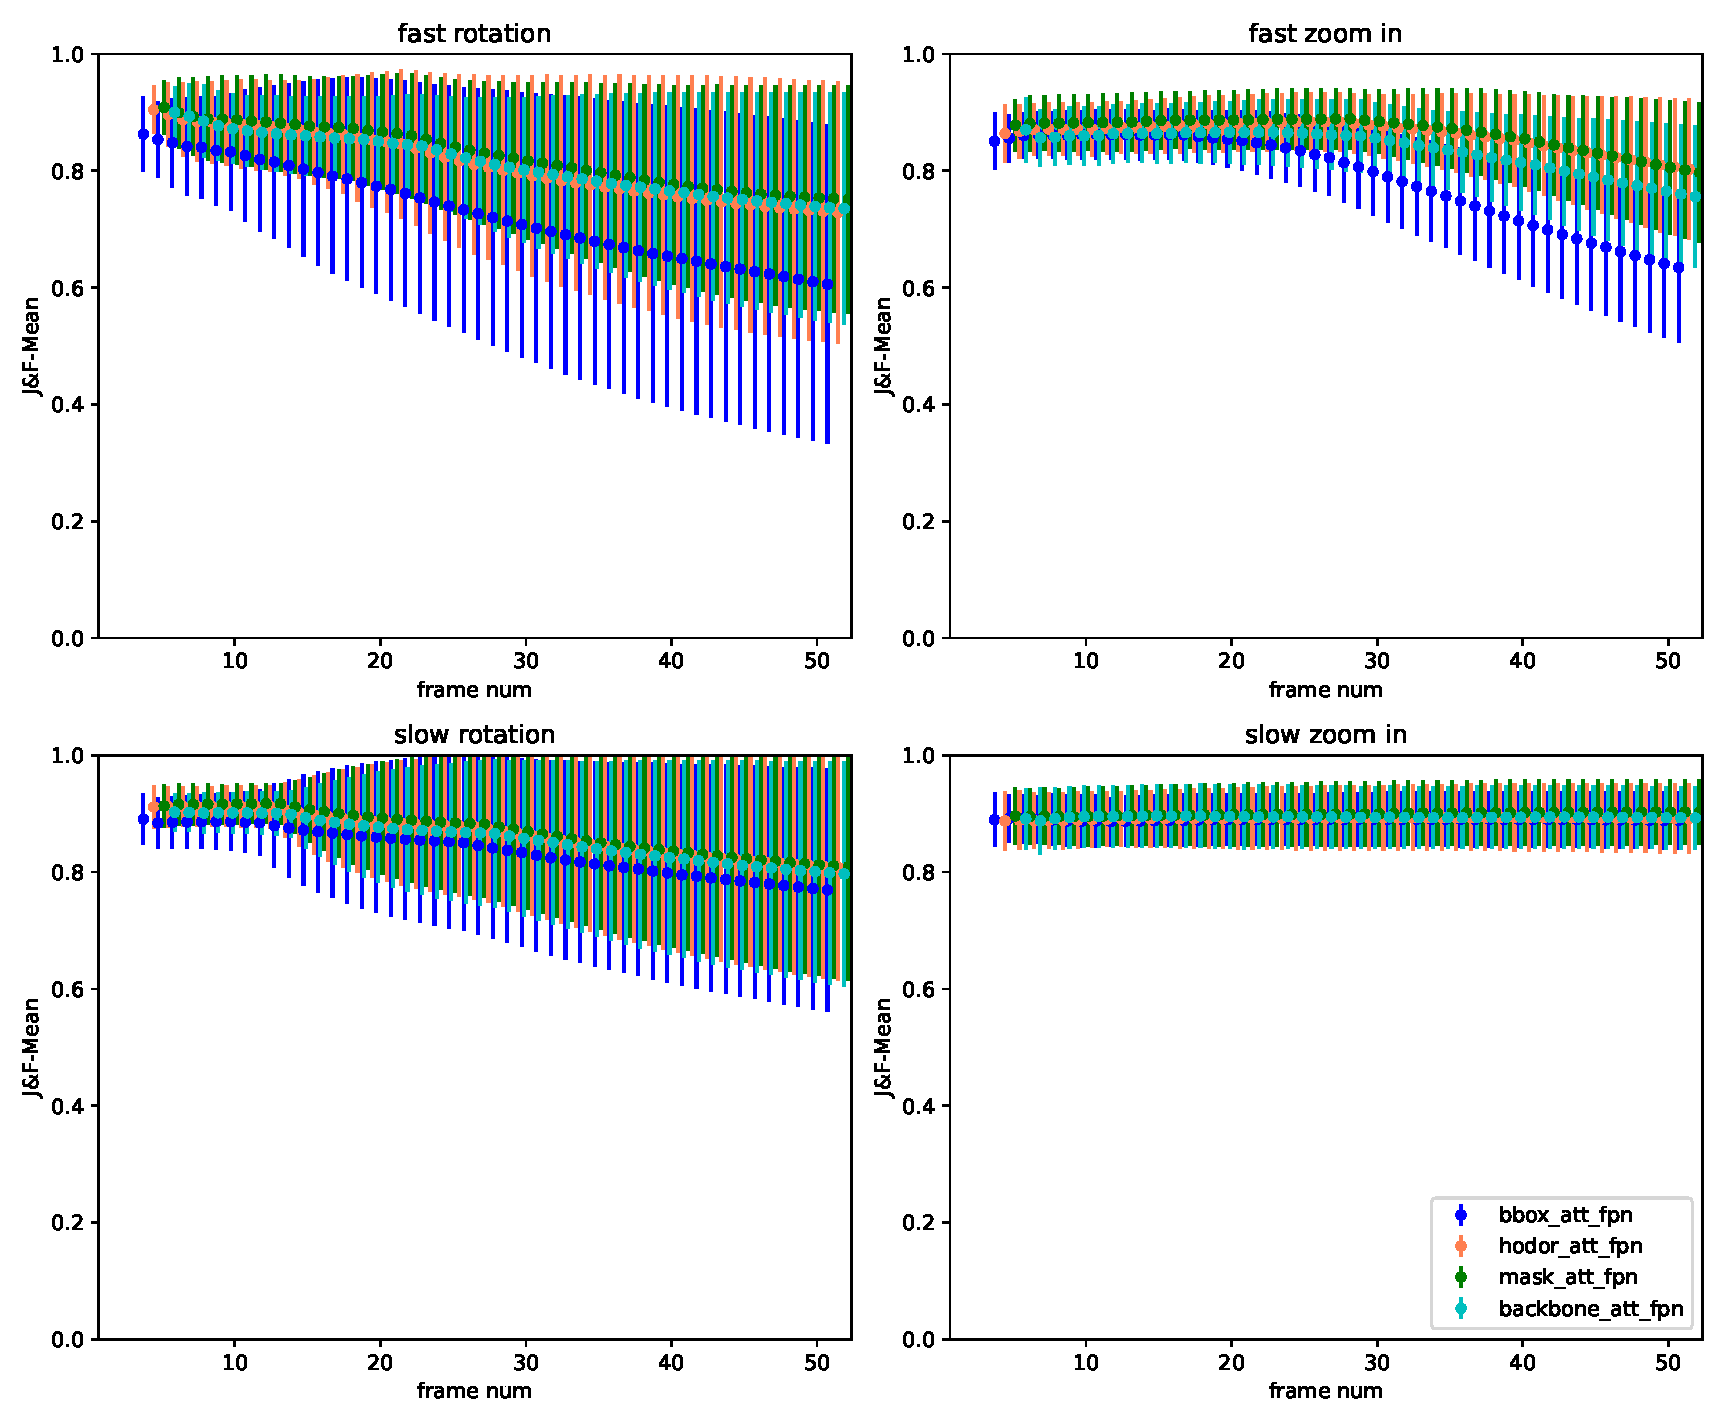
\includegraphics[width=1.\linewidth]{figures/04_experiments/encoder_ablations/bbox_att_fpn-hodor_att_fpn-mask_att_fpn-backbone_att_fpn-movement_all_variance.pdf}
    \caption{Temporal analysis of encoder variants (with variance)}
    \label{fig:all_encoders_var}
    
\end{figure}

Observing \figref\ref{fig:all_encoders}, we note that in easier scenes, where the camera movement does not result in dramatic changes in object appearance (slow zoom in), all encoders perform comparably well in terms of the mean achieved $J\&F$ score, even when taking into account the performance variance in \figref\ref{fig:all_encoders_var}. However, things appear to become critical in cases where the camera velocity increases. Both in case of a rotational and translational camera movement with fast velocity, the bounding box encoder performance drops dramatically as the sequence increases in length. It is worth noting that all methods' performance drops in fast scenes, probably due to accumulation of propagated errors over time, as the model performs inference on a long scene. Still, the bounding box encoder appears to be more affected in terms of performance as time progresses, which renders this model variant only suitable for cases where the movement is slow and controlled. \par

\subsubsection{Corner case analysis}

To better highlight the differences in behaviour between different encoder types, a 'crowdness/cluttereness' analysis was performed, to investigate the role of occlusions and cluttereness in the performance drop in difficult scenarios. For this analysis, the focus was placed on particularly difficult scenes, specifically the challenging 'fast rotation' sequence subgroup, based on the temporal behaviour of all encoder types summarized in  \figref\ref{fig:all_encoders}. For the 10 sequences belonging to this subgroup, the $J\&F$ score, the visibility score, computed according to \eqref{eq: visibility score}, and the number of objects present were plotted for 50 frames. The plots involving all 10 scenes can be found in \autoref{seq: appendix_croudness} in the Appendix. \par

A more readable version of the plots in \autoref{seq: appendix_croudness} is obtained by performing a corner case analysis. Specifically,  for each past frame encoder type, the sequence with the largest and the smallest drop in performance indicated by the $J\&F$ mean was plotted along with the visibility score and the number of objects in the scene. To further ease the plot readability, the number of samples is only indicated in case it changes, otherwise it is only plotted with a rhombus in the first frame. \par


\vspace{3mm}

\begin{figure} [ht!]
    \centering
    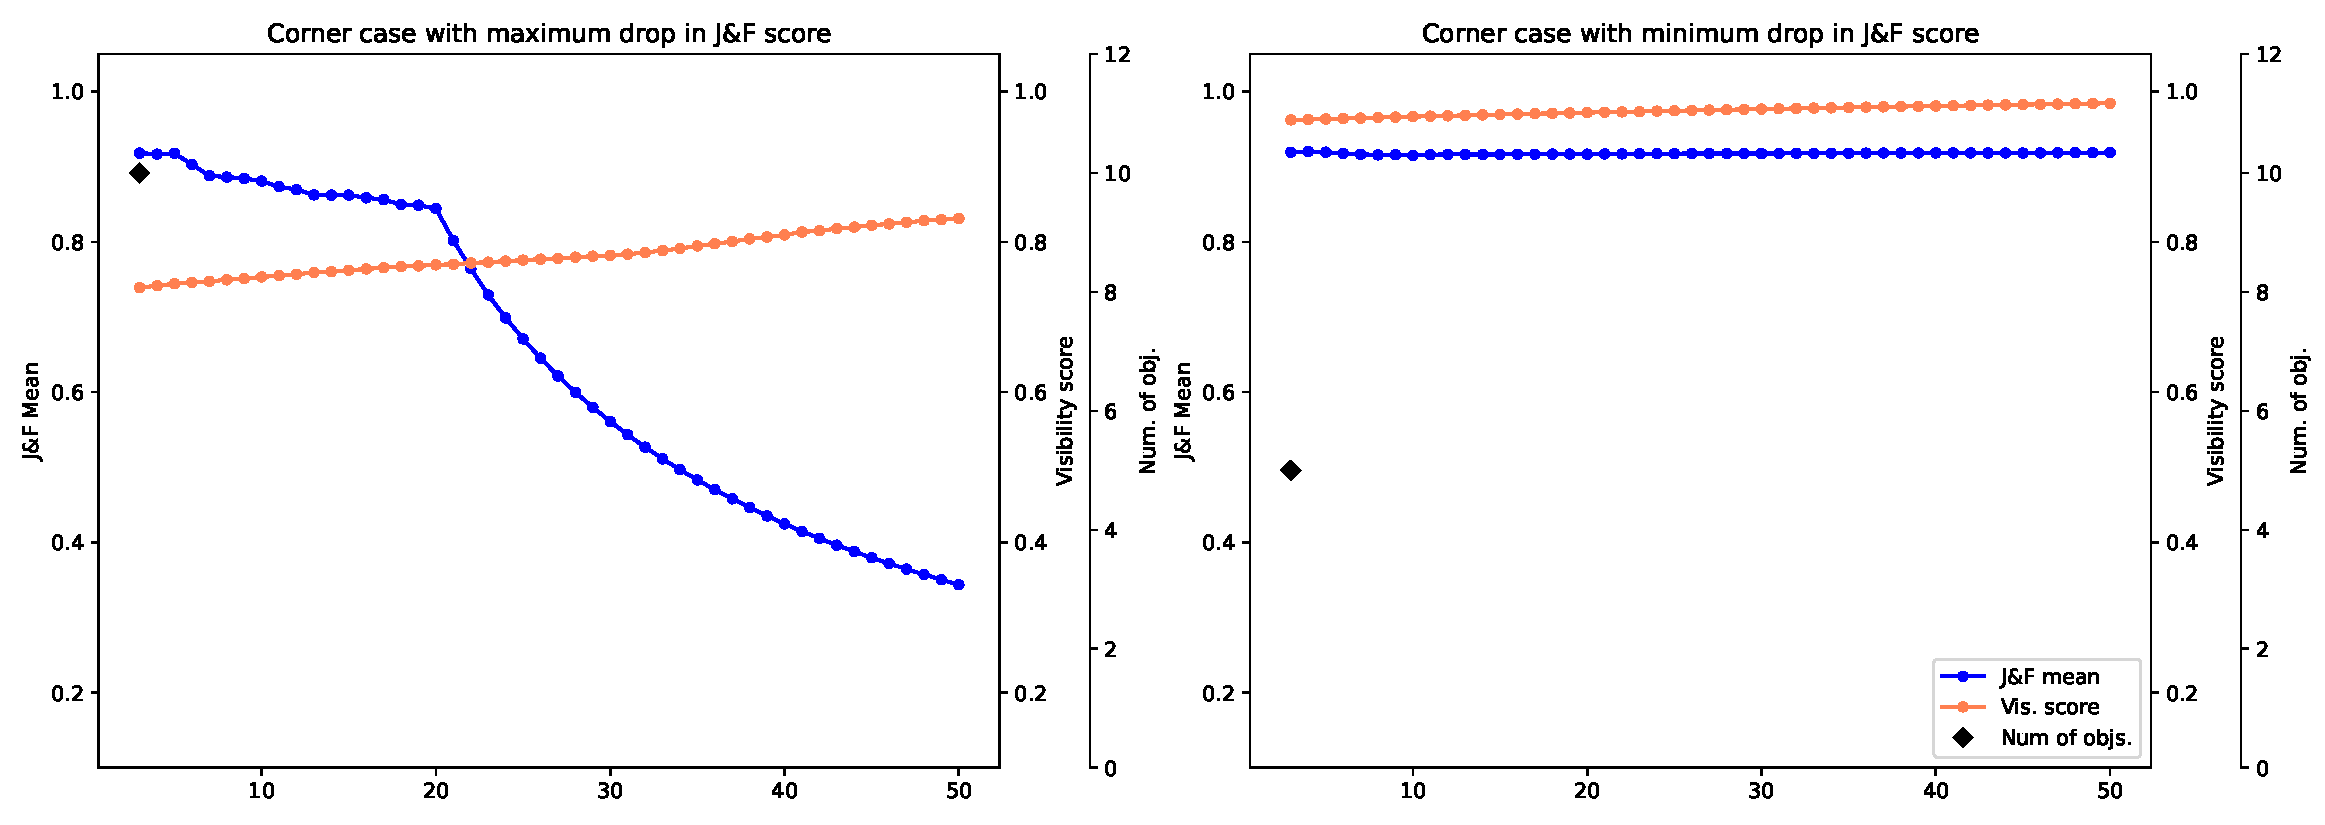
\includegraphics[width=1.\linewidth]{figures/04_experiments/corner_cases_ablations/9_backbone_att_fpn_fast_rotation-corner_cases.pdf}
    \caption{Corner case analysis for the backbone encoder}
    \label{fig:corner_cases1}
    
\end{figure}
\begin{figure}[ht!]
    \centering
    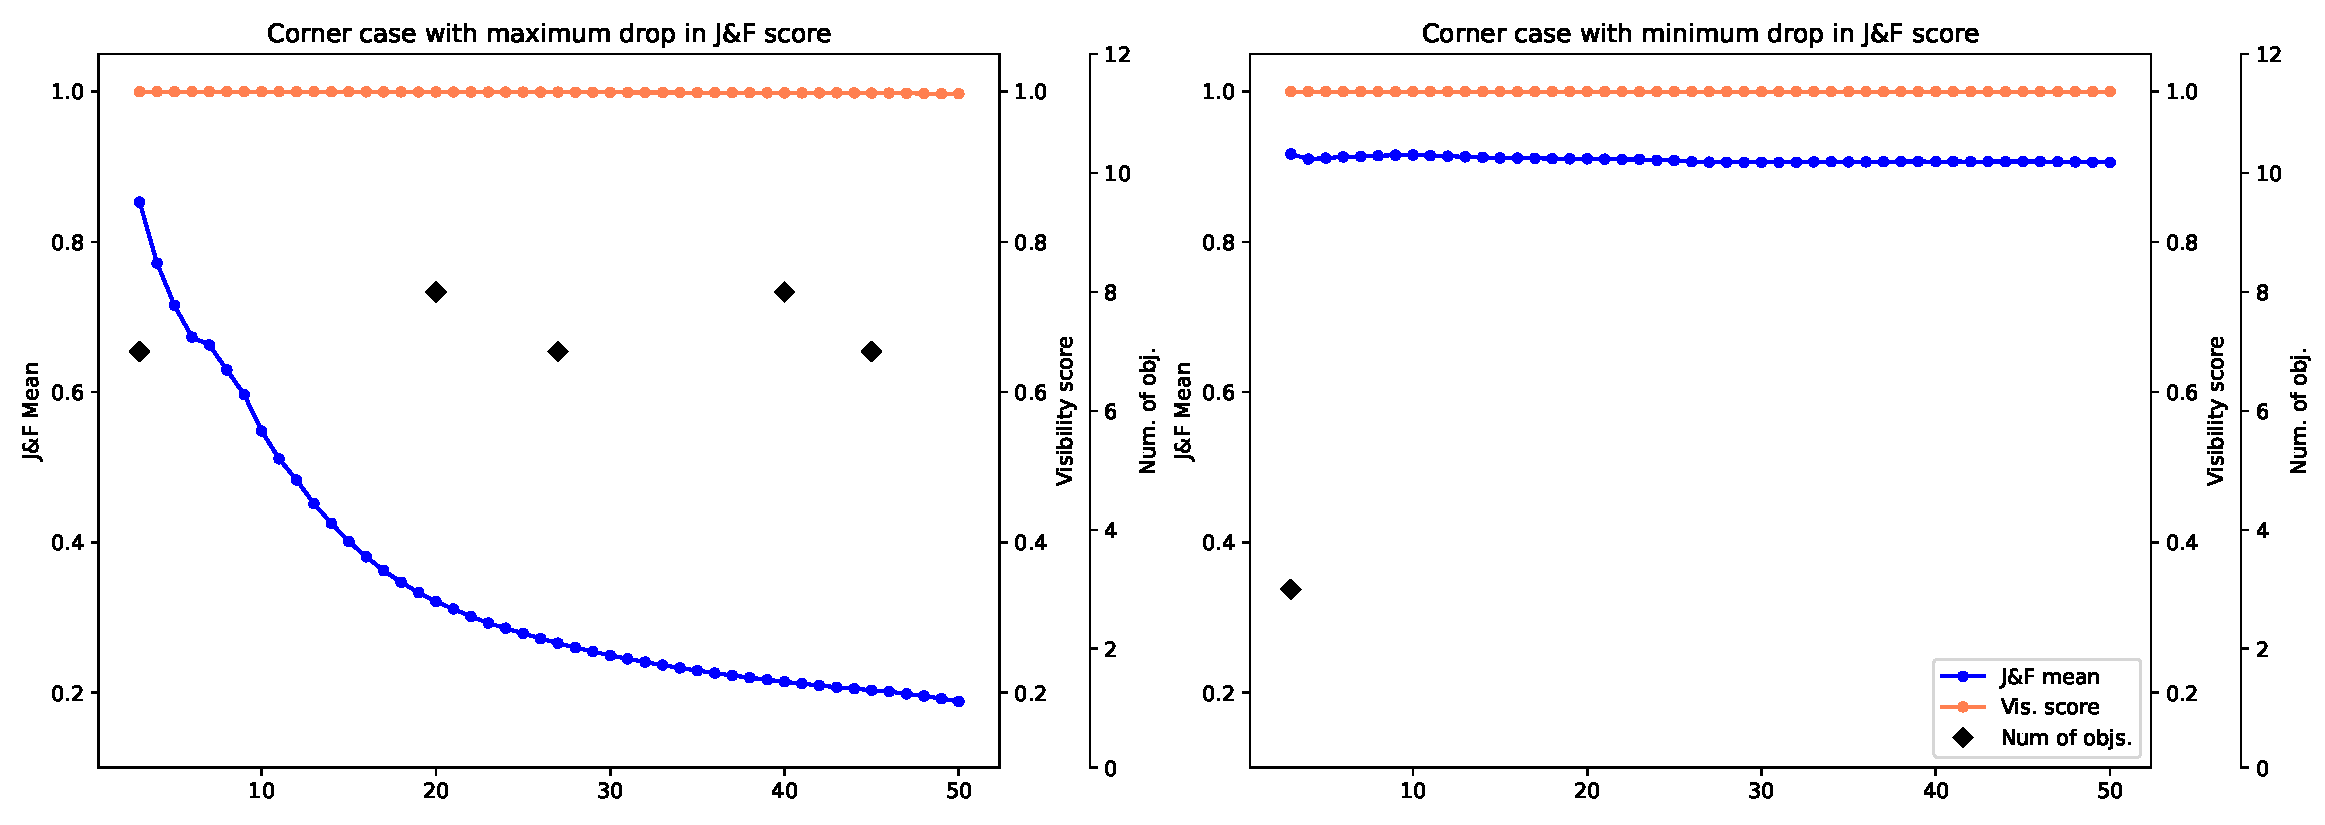
\includegraphics[width=1.\linewidth]{figures/04_experiments/corner_cases_ablations/5_bbox_att_fpn_fast_rotation-corner_cases.pdf}
    \caption{Corner case analysis for the bounding box encoder}
    \label{fig:corner_cases2}
    
\end{figure}



\begin{figure}[ht!]
    \centering
    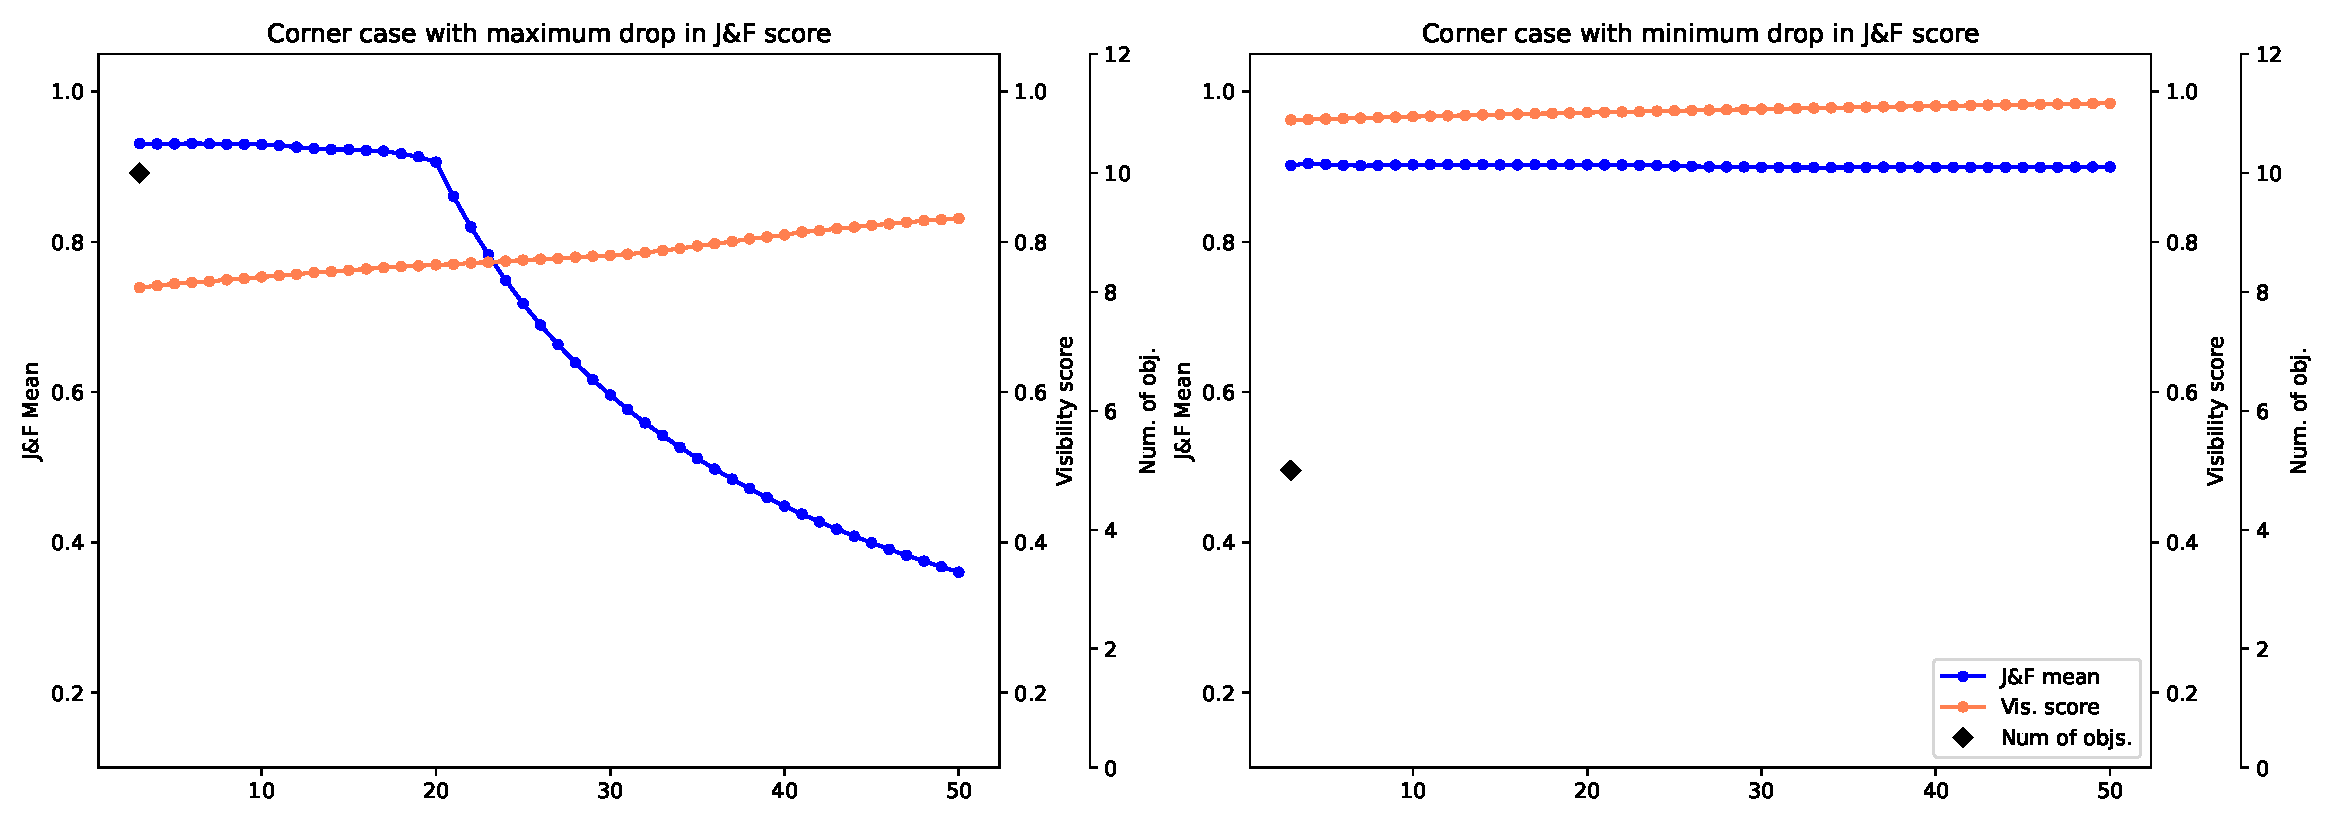
\includegraphics[width=1.\linewidth]{figures/04_experiments/corner_cases_ablations/6_mask_att_fpn_fast_rotation-corner_cases.pdf}
    \caption{Corner case analysis for the mask encoder }
    \label{fig:corner_cases4}
    
\end{figure}

Comparing the plots in \figref\ref{fig:corner_cases1}, \figref\ref{fig:corner_cases2} and \figref\ref{fig:corner_cases4}, it becomes evident that all methods struggle with very crowded scenes where a large number of objects is present. For the backbone and the mask encoders, the most difficult scene involves a large number of objects (10 objects) combined with a low visibility score (<0.8), which implies that some of these objects are partially occluded by other objects in the scene, an indication of increased clutterness. On the contrary, both aforementioned encoders perform best in scenes with a relatively small number of objects (5 objects), no disappearances and a visibility score close to 1.0, which indicates that the objects are scattered far apart in the scene. Hence, both the backbone encoder and the mask encoders deal more easily with the appearance changes imposed to objects due to the camera movement, if the objects are far apart and easy to distinct. On the other hand, the bounding box encoder seems to struggle in a scene with an object disappearance, even though the rest of the objects are clearly visible and most probably far apart with a visibility score of 1. It also appears that the number of objects in the scene plays a more important role than how distinct the objects are in terms of their physical distance, as it performs best in a scene with only 2 objects. \par
\newpage
Another important observation from the cluttereness analysis plots is that more sophisticated, appearance based methods (backbone encoder, mask encoder) seem to retain a relatively good performance for more frames ($\sim$ 20 frames), before the $J\&F$ score begins to drop after the 20th frame. In contrast, the performance drop of the bounding box encoder in its most challenging scene begins at t=1 and continues dramatically until the end of the scene. \par

\subsection{Matching comparisons}


For the matching type comparisons, three options were included in the analysis, all combined with the same encoder and decoder. More specifically, the mask encoder without mean was selected for past frame encoding, since it demonstrates best performance and retains best performance in the course of time even in challenging scenes (see \figref\ref{fig:all_encoders}). For the decoder, the standard FPN option was kept in all experiments in this subsection. The matching options involved in the analysis are matching by separable attention, e-step matching, which is a version GMM matching with only a single e-step of the EM algorithm performed, and GMM matching with 5 EM algorithm iterations. As mentioned in \autoref{chapter:method}, the number of iterations for the EM algorithm is defined as a hyperparameter.\par

\begin{figure}[ht!]
    \centering
    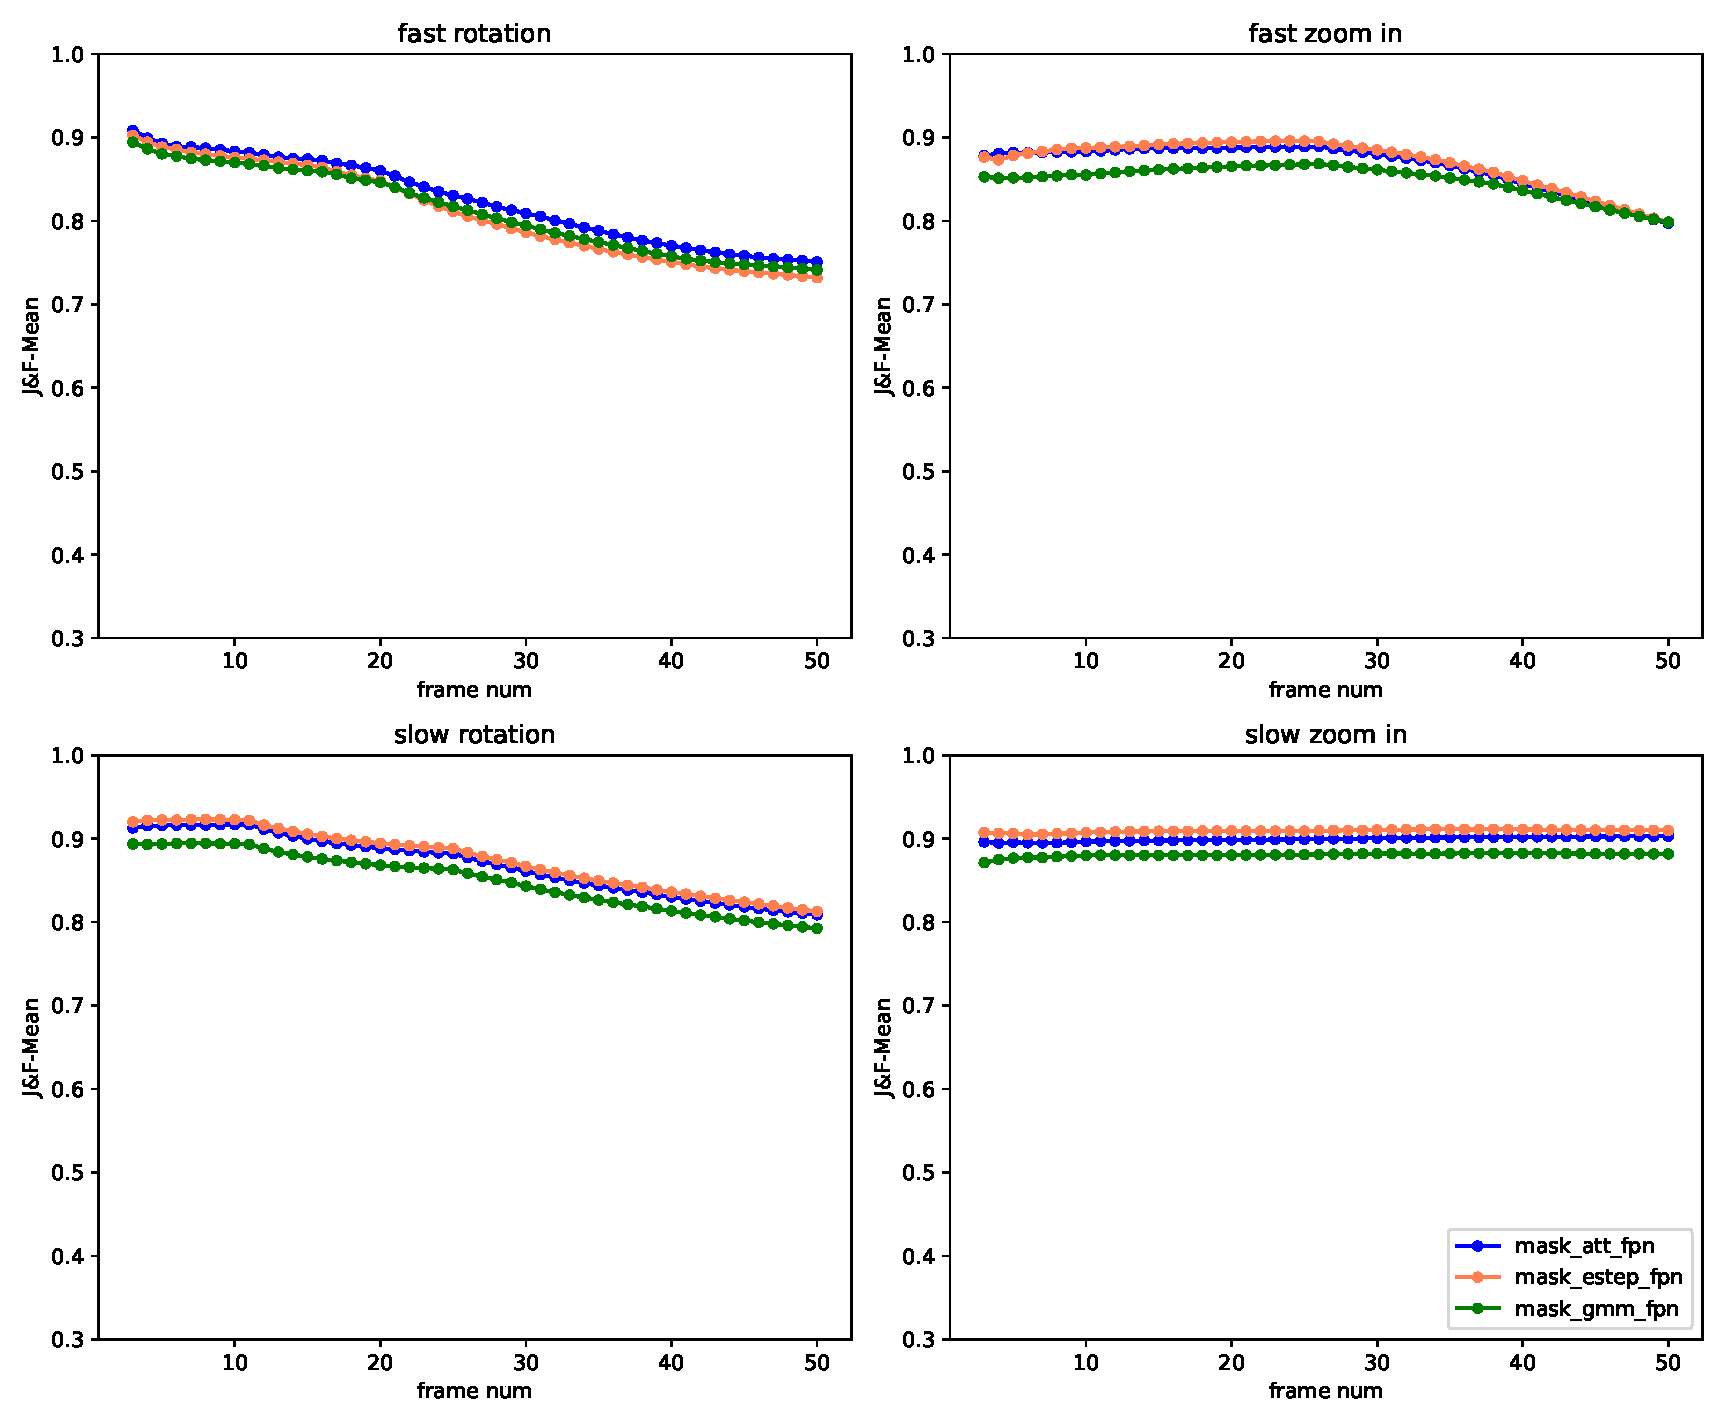
\includegraphics[width=1.\linewidth]{figures/04_experiments/matching_ablations/mask_att_fpn-mask_estep_fpn-mask_gmm_fpn-movement_all.pdf}
    \caption{Temporal analysis of matching type variants}
    \label{fig:matching_ablations_all}
    
\end{figure}
\begin{table}[h!]
\caption{Comparison of matching types}
\centering
\begin{tabular}{|c|ccc|ccc|c|c|c|}
\hline
\multicolumn{1}{|c|}{\multirow{2}{*}{Matching}} & 
 \multicolumn{3}{c|}{Tracking Dataset}                     & \multicolumn{3}{c|}{Davis} & \multicolumn{1}{c|}{\multirow{2}{*}{time [s]}} & \multicolumn{1}{c|}{\multirow{2}{*}{GPU}} &
 \multicolumn{1}{c|}{\multirow{2}{*}{Lrn. Par.}} \\ \cline{2-7} 
 \multicolumn{1}{|c|}{} &
 \multicolumn{1}{c|}{J} & \multicolumn{1}{c|}{F} & \multicolumn{1}{c|}{J\&F} & \multicolumn{1}{c|}{J} & \multicolumn{1}{c|}{F} & \multicolumn{1}{c|}{J\&F} &\multicolumn{1}{c|}{} &\multicolumn{1}{c|}{} 
 &\multicolumn{1}{c|}{} \\ \hline

attention  & 0.718 & 0.808 & 0.763 &  0.438 & 0.524 & 0.481 &   0.0709  &  1.255Gb & 45.3M  \\ 

estep  & 0.711 & 0.799 & 0.755 & 0.486 & 0.570 & 0.524 & 0.0727  & 423Mb & 45.2M  \\                   

GMM   & 0.702  & 0.802  &  0.752 & 0.416 & 0.468 & 0.439 & 0.0764 & 443Mb &  45.2M  \\ \hline

\end{tabular}
 \label{Tab:matching_ablations}
\end{table}

\vspace{7mm}

 Taking into account solely the performance on our test set, all methods perform comparably well, even when considering the temporal aspect and the variance in the overall performance (see  \figref\ref{fig:matching_ablations_all} and \figref\ref{fig:matching_ablations_all_variance}). On the cross domain evaluation set DAVIS, e-step matching seems to perform better than attention-based matching. This observation agrees with our intuition 
 %\comWB{did you specify that somewhere} 
 that GMM matching may result in a tracker less prone to overfitting to the specific training set it was optimised on, since the GMM matching block, unlike attention, does not involve learnable parameters. The role of GMM matching during training is merely to help optimise the input image encoder to extract features that are more suitable for identifying objects in different scenes. Hence, even though involving learnable parameters in the matching process evidently boosts performance in the domain the network is trained on, it is questionable whether the relation between features from different frames highlighted with attention is a similarity function as universal as the Gaussian Mixture assumption.
 %\comWB{not quite clear}. 
 Though not further examined in the course of this thesis, we think that an explainability analysis on the matching learned by the attention block in the proposed network could serve as interesting future work.
 \par


\begin{figure}[ht!]
    \centering
    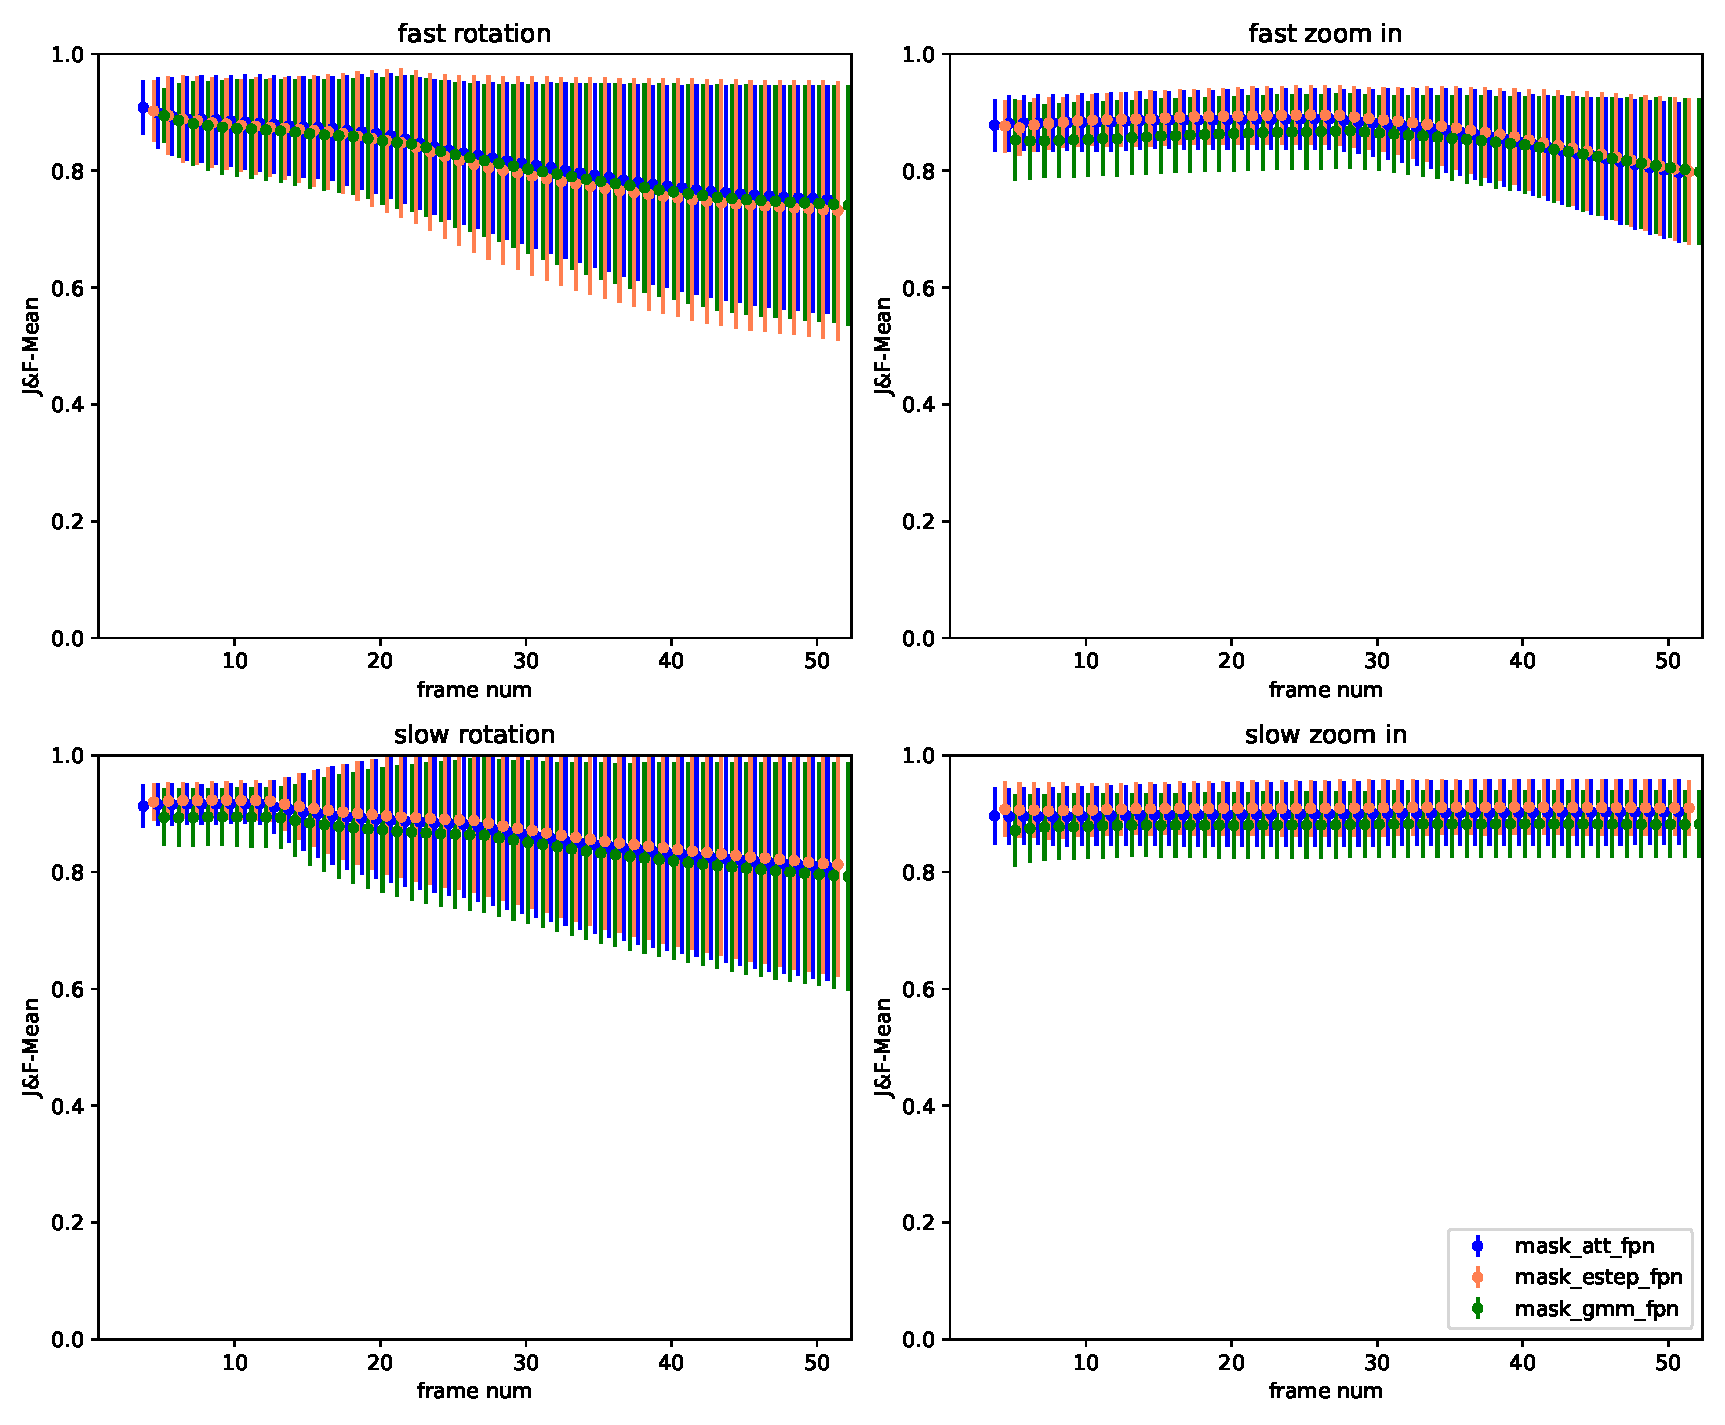
\includegraphics[width=1.\linewidth]{figures/04_experiments/matching_ablations/mask_att_fpn-mask_estep_fpn-mask_gmm_fpn-movement_all_variance.pdf}
    \caption{Temporal analysis of matching type variants (with variance)}
    \label{fig:matching_ablations_all_variance}
    
\end{figure}
\newpage
Apart from purely performance-based criteria, an efficiency analysis was performed on all three options. In terms of inference time, the efficient separable attention proposed is faster than the other two options, probably due to the high parallelism of purely tensor-based operations involved in the method that run optimally with PyTorch. The GMM options on the other hand with the for loop introduced by the EM algorithm appears to require more time to execute. Since GMM matching is still a work in progress, the inference time is expected to decrease in a more mature version of the method and is left open as a research question. However, in terms of GPU allocation, the GMM variant is far less costly than attention. This difference in GPU allocation confirms the intuition described in \autoref{chapter:method} that the GMM based matcher is more lightweight and hence more suitable for expanding in a more elaborate multi-scale matching variant. The expansion of GMM matching in its multi scale counterpart is explored in subsection 3.3.4.
\subsection{Decoder comparisons}

Apart from the encoder and matching type comparisons, different decoders were tested with regard to their performance under the same setup. Similarly to the matching type comparison, the mask encoder without mean was used for past feature encoding in all experiments in this subsection. Regarding matching, the GMM-based matching was utilised in all compared model variants, because it is the only option compatible with all decoders discussed in this work, including the responsibility upsampler. Under this setup, the FPN decoder, the MLP decoder and the responsibility upsampler are compared primarily in view of their performance, but also in terms of their inference time. \par

\begin{table}[ht!]
\caption{Comparison of decoder types }
\centering
\begin{tabular}{|c|ccc|ccc|c|}
\hline
\multicolumn{1}{|c|}{\multirow{2}{*}{Decoder Type}} & \multicolumn{3}{c|}{Tracking Dataset} & \multicolumn{3}{c|}{Davis} 
& \multicolumn{1}{c|}{\multirow{2}{*}{time [s]}} \\ \cline{2-7} 
\multicolumn{1}{|c|}{}  & \multicolumn{1}{c|}{J} & \multicolumn{1}{c|}{F} & \multicolumn{1}{c|}{J\&F}  & \multicolumn{1}{c|}{J} & \multicolumn{1}{c|}{F} & \multicolumn{1}{c|}{J\&F} &\multicolumn{1}{c|}{}   \\ \hline

fpn  &  0.702 &  0.802 &  0.752  &  0.416  & 0.468  &  0.439  &  0.0764 \\ 
%\cline{1-1}
mlp         &  0.707      & 0.781   &  0.744     &  0.373 &  0.488  &  0.43  &  0.0741  \\ %\cline{1-1}

resp. decoder   &  0.624  &   0.677  & 0.650   &  0.364  &  0.384 & 0.374 & 0.1032  \\ \hline

\end{tabular}
 \label{Tab:decoder_ablations}
\end{table}

\begin{figure}[ht!]
    \centering
    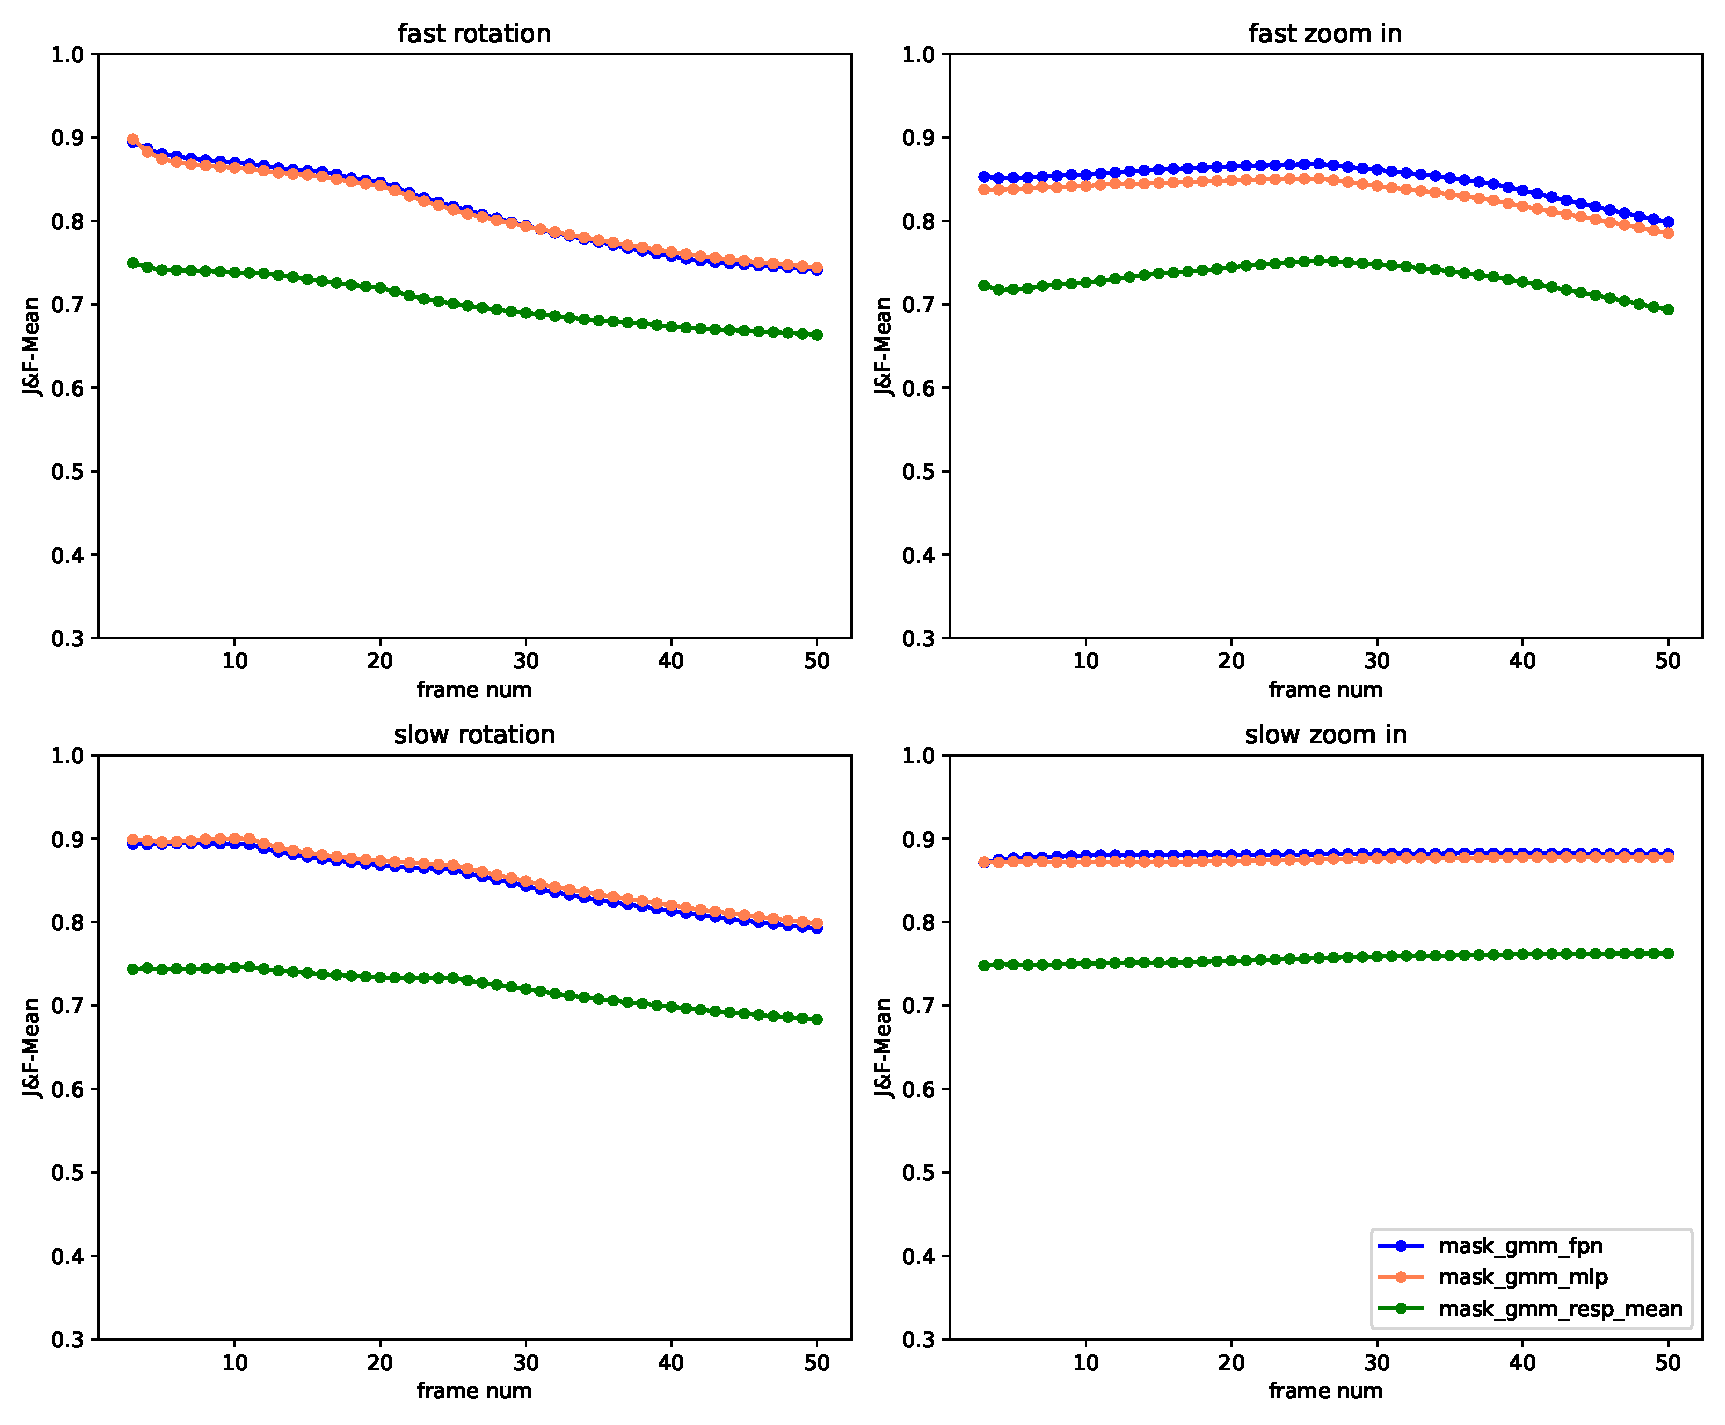
\includegraphics[width=1.\linewidth]{figures/04_experiments/decoder_ablations/mask_gmm_fpn-mask_gmm_mlp-mask_gmm_resp_mean-movement_all.pdf}
    \caption{Temporal analysis of decoder variants}
    \label{fig:decoder_abl_all}
    
\end{figure}






Starting the analysis on our own synthetic dataset, we note that there is an important performance gap between the FPN/MLP solution and the responsibility upsampler. This result agrees with our expectations, since the responsibility upsampler directly decodes the matched feature maps after the matching block and does not involve any more layers with learnable parameters that can perform some sort of filtering, that typically results in more refined predictions. The performance gap is evident in both the area based metric $J$, but also the contour focused metric F, in both our test set and the DAVIS evaluation, see \tabref\ref{Tab:decoder_ablations}. Moreover, even in terms of inference time the responsibility upsampler is more costly, since multiple GMM heads are required to achieve a relatively good performance. So, as expected, the responsibility upsampler is not the optimal choice in view of solely performance or computational efficiency based criteria. However, as already mentioned in chapter 3, the responsibility upsampler provides more interpretable (due to their probabilistic nature) predictions, which may be a desirable aspect in various use cases. \par

% Furthermore, the responsibility upsampler can be regarded as future work that 
% \par

Between the FPN and the SegFormer MLP-based decoder the performance gap is quite small. However, it seems that the pyramid multi-scale decoder architecture of the FPN still poses an advantage to the purely MLP based decoder from \parencite{segformer}.
\vspace{10mm}
\begin{figure}[ht!]
    \centering
    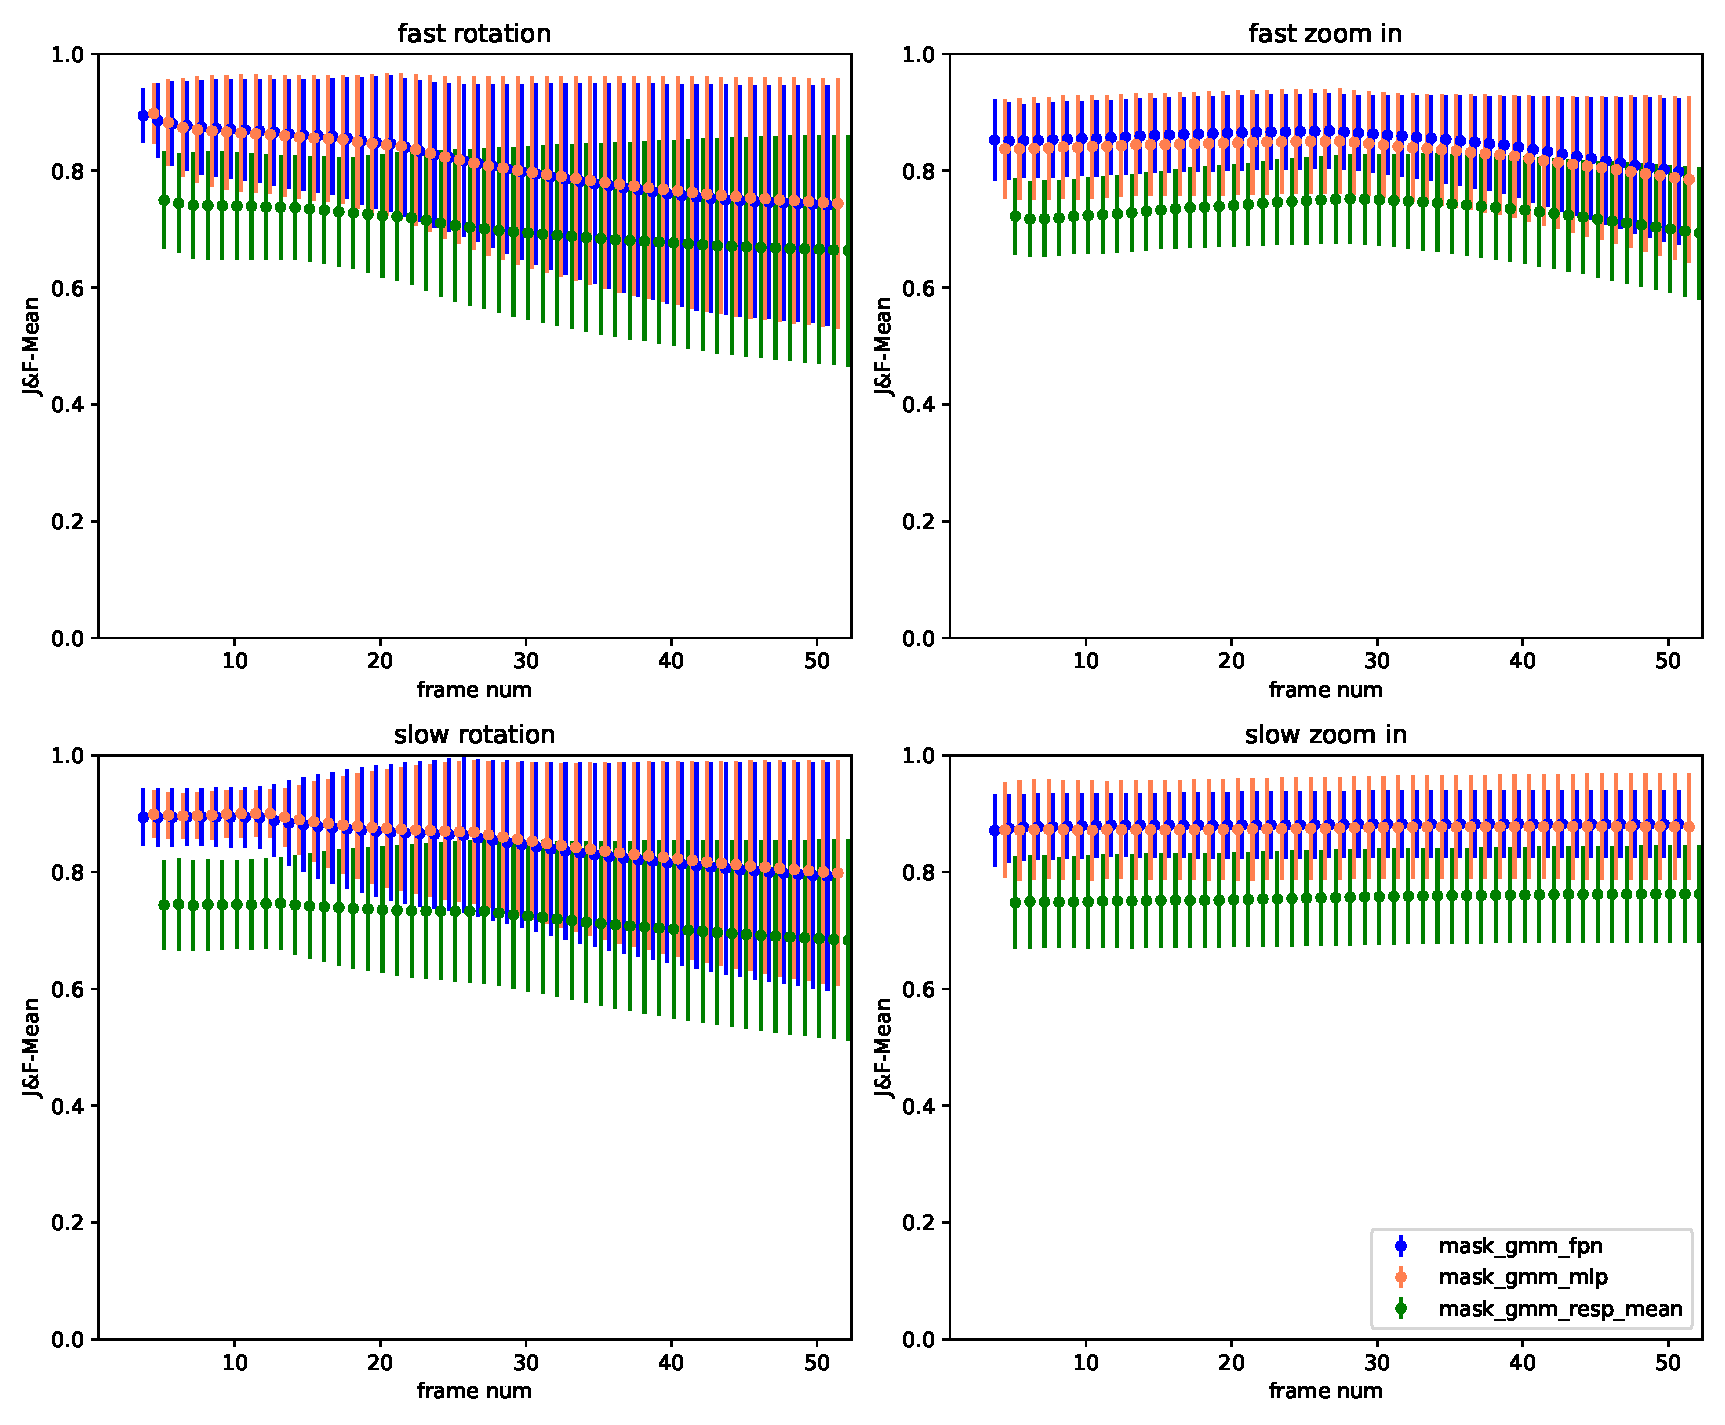
\includegraphics[width=1.\linewidth]{figures/04_experiments/decoder_ablations/mask_gmm_fpn-mask_gmm_mlp-mask_gmm_resp_mean-movement_all_variance.pdf}
    \caption{Temporal analysis of decoder variants (with variance)}
    \label{fig:decoder_abl_all_variance}
    
\end{figure}
\clearpage

\subsection{Comparison with multi-scale matching and multiple object descriptors}

The final preliminary experiment described in this section is an attempt to expand GMM matching to a  multi-scale variant. Both the backbone and mask encoder follow or have the potential to be expanded to a hierarchical structure since they build upon the SegFormer-B3 backbone for past feature encoding. However, matching so far has only been performed on the smallest feature map scale provided at the output of the encoder (1/32 of the original input image). Since hierarchical (Swin, \cite{swin}, SegFormer, \cite{segformer}) and pyramid structures (FPN, \cite{fpn}) have proven to be beneficial for model performance, the question emerged whether multi-scale matching on all features in the respective resolutions can improve the performance of the proposed method. \par

\begin{table}[ht!]
\caption{Comparison of single-scale with multi-scale matching}
\centering
\label{tab:multires}
\begin{tabular}{|c|ccc|ccc|c|}
\hline
\multicolumn{1}{|c|}{\multirow{2}{*}{Matching Type}} & \multicolumn{3}{c|}{Tracking Dataset}                                              & \multicolumn{3}{c|}{Davis} &\multicolumn{1}{c|}{\multirow{2}{*}{Time [s]}}                                                         \\ \cline{2-7} 
\multicolumn{1}{|c|}{}                              & \multicolumn{1}{c|}{J} & \multicolumn{1}{c|}{F} & \multicolumn{1}{c|}{J\&F}  & \multicolumn{1}{c|}{J} & \multicolumn{1}{c|}{F} & \multicolumn{1}{c|}{J\&F}  & \multicolumn{1}{c|}{}                               \\ \hline

Mask enc. single-scale &   0.702 &  0.802 & 0.752  &  0.416  & 0.468  &  0.439 & 0.0764  \\ 
%\cline{1-1}
Mask enc. multi-scale &  0.702 &  0.786 & 0.744  & 0.399 & 0.478 & 0.438 & 0.1030 \\ %\cline{1-1}

Mask enc. multi-scale + descr   &  0.722 &   0.802 & 0.762  & 0.497  & 0.584 & 0.541 & 0.1340\\ \hline

\end{tabular}
\end{table}
Though expanding the patch encoder and the matcher to multiple feature scales seems intuitive, the computational cost of this operation immediately explodes, depending on the nature of the matching operation performed.
%\comWB{can you say how much?}
For example, more elaborate architectures like HODOR \parencite{athar2022hodor} that involve self-attention on the past extracted features and perform a computationally intensive attention operation for matching (masked attention instead of our separable attention) cannot be expanded to a multi-scale variant, without a significant cost on computational resources. We considered more reasonable to expand the GMM matcher to multi-scale version, because it requires less GPU allocation compared to our separable attention and can be seen as more lightweight in that regard. \par

Apart from expanding matching to all extracted feature scales, a further attempt to boost performance would be to initialise multiple descriptors (clusters) for each object and the background class. More specifically, in this experiment 8 descriptors were initialised for the background class and 2 for each object. Especially, for the background class, we expect this choice to be very beneficial for performance, particularly in scenes where objects similar to the ones that are tracked are expected to be treated as background. By allowing the model to learn multiple descriptors for the background in scenes where objects are expect to be ignored, we expect the model to achieve better object of interest/ background separation. Our intuition is indeed verified by the preliminary results, see \tabref\ref{tab:multires}. \par
\begin{figure}[ht!]
    \centering
    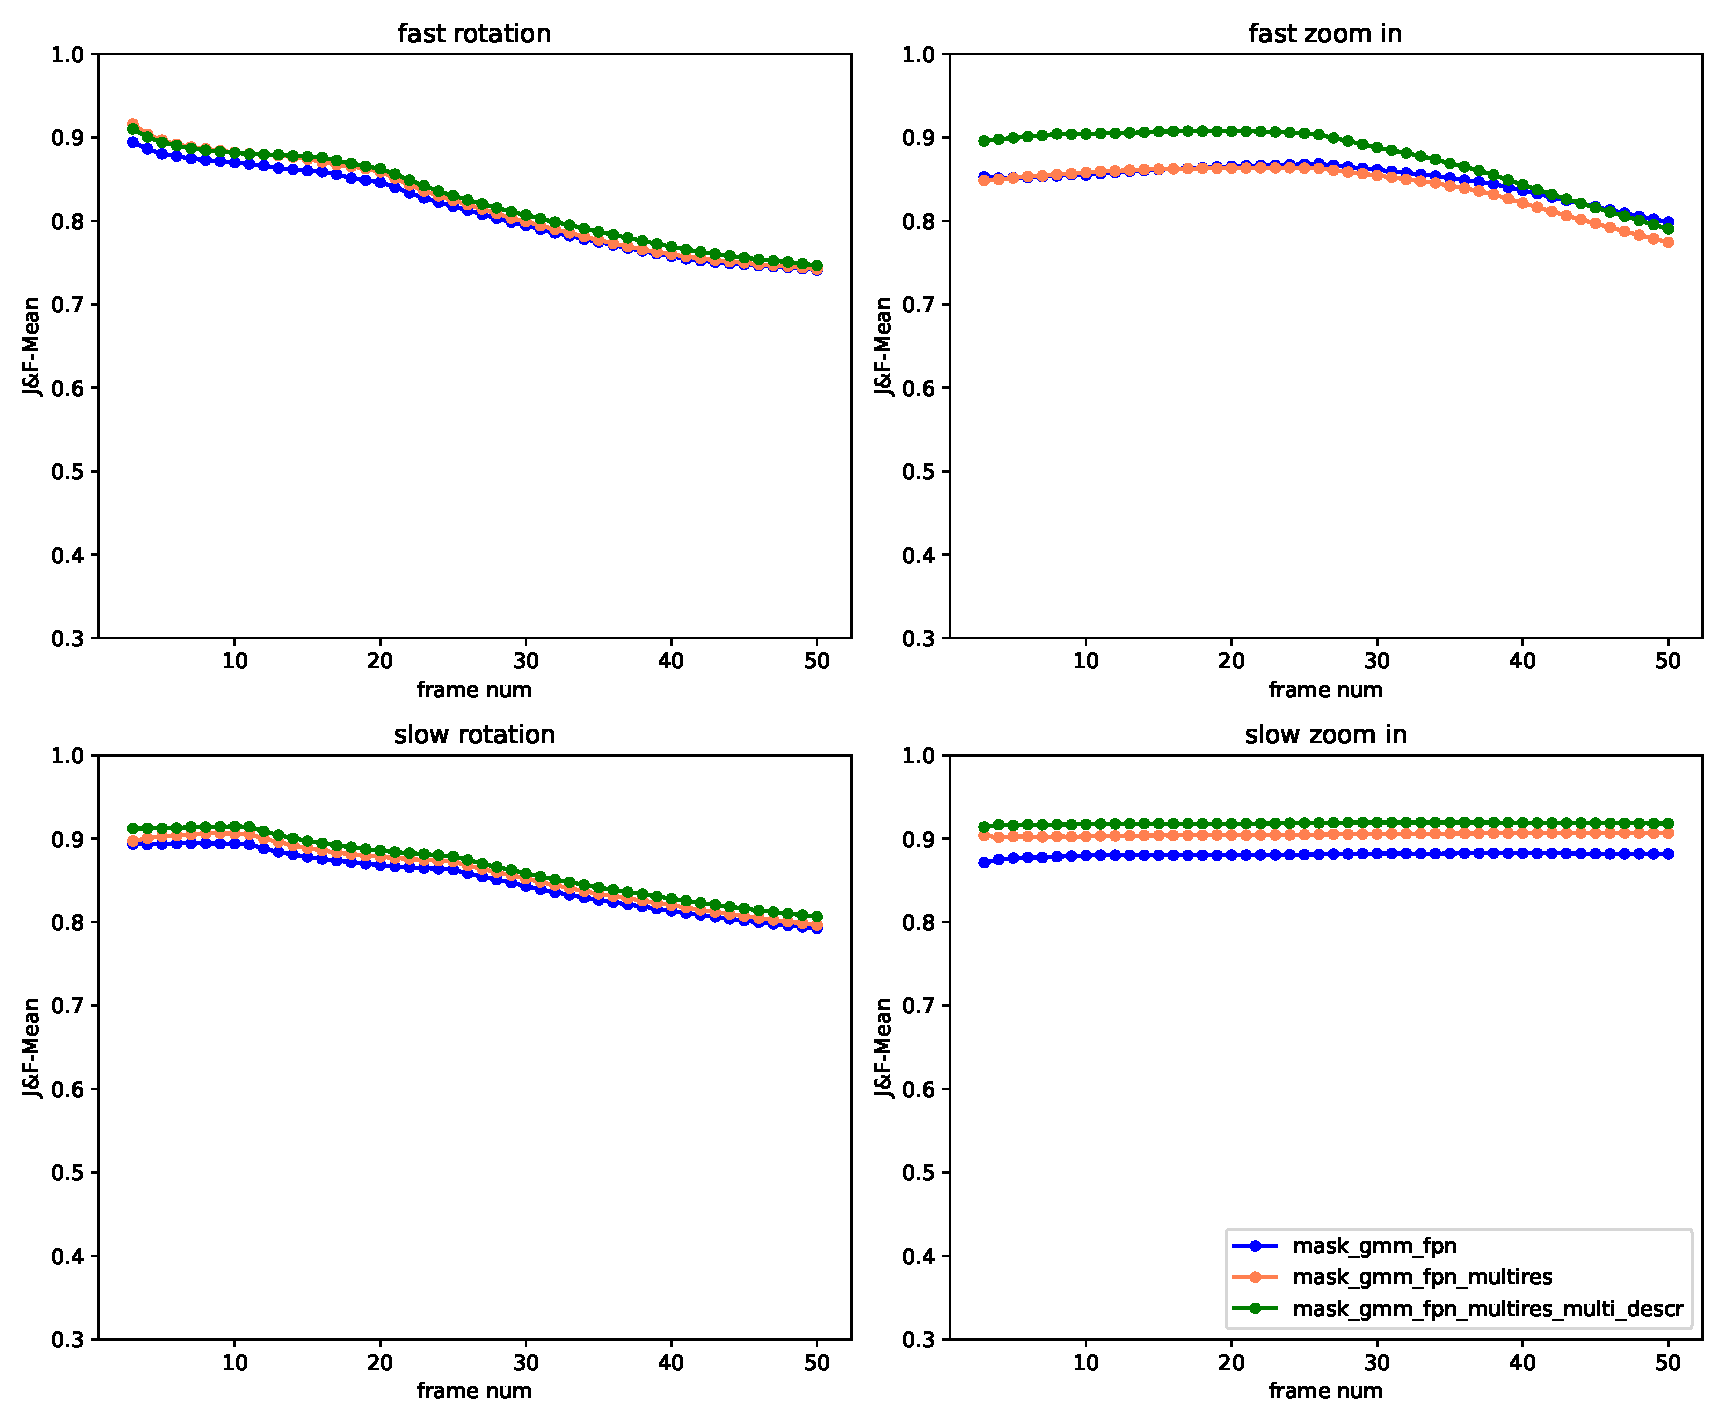
\includegraphics[width=1.\linewidth]{figures/04_experiments/multires_comparisons/mask_gmm_fpn-mask_gmm_fpn_multires-mask_gmm_fpn_multires_multi_descr-movement_all.pdf}
    \caption{Temporal analysis of single- vs multi-scale matching variants}
    \label{fig:multires_abl_all}
    
\end{figure}


\begin{figure}[ht!]
    \centering
    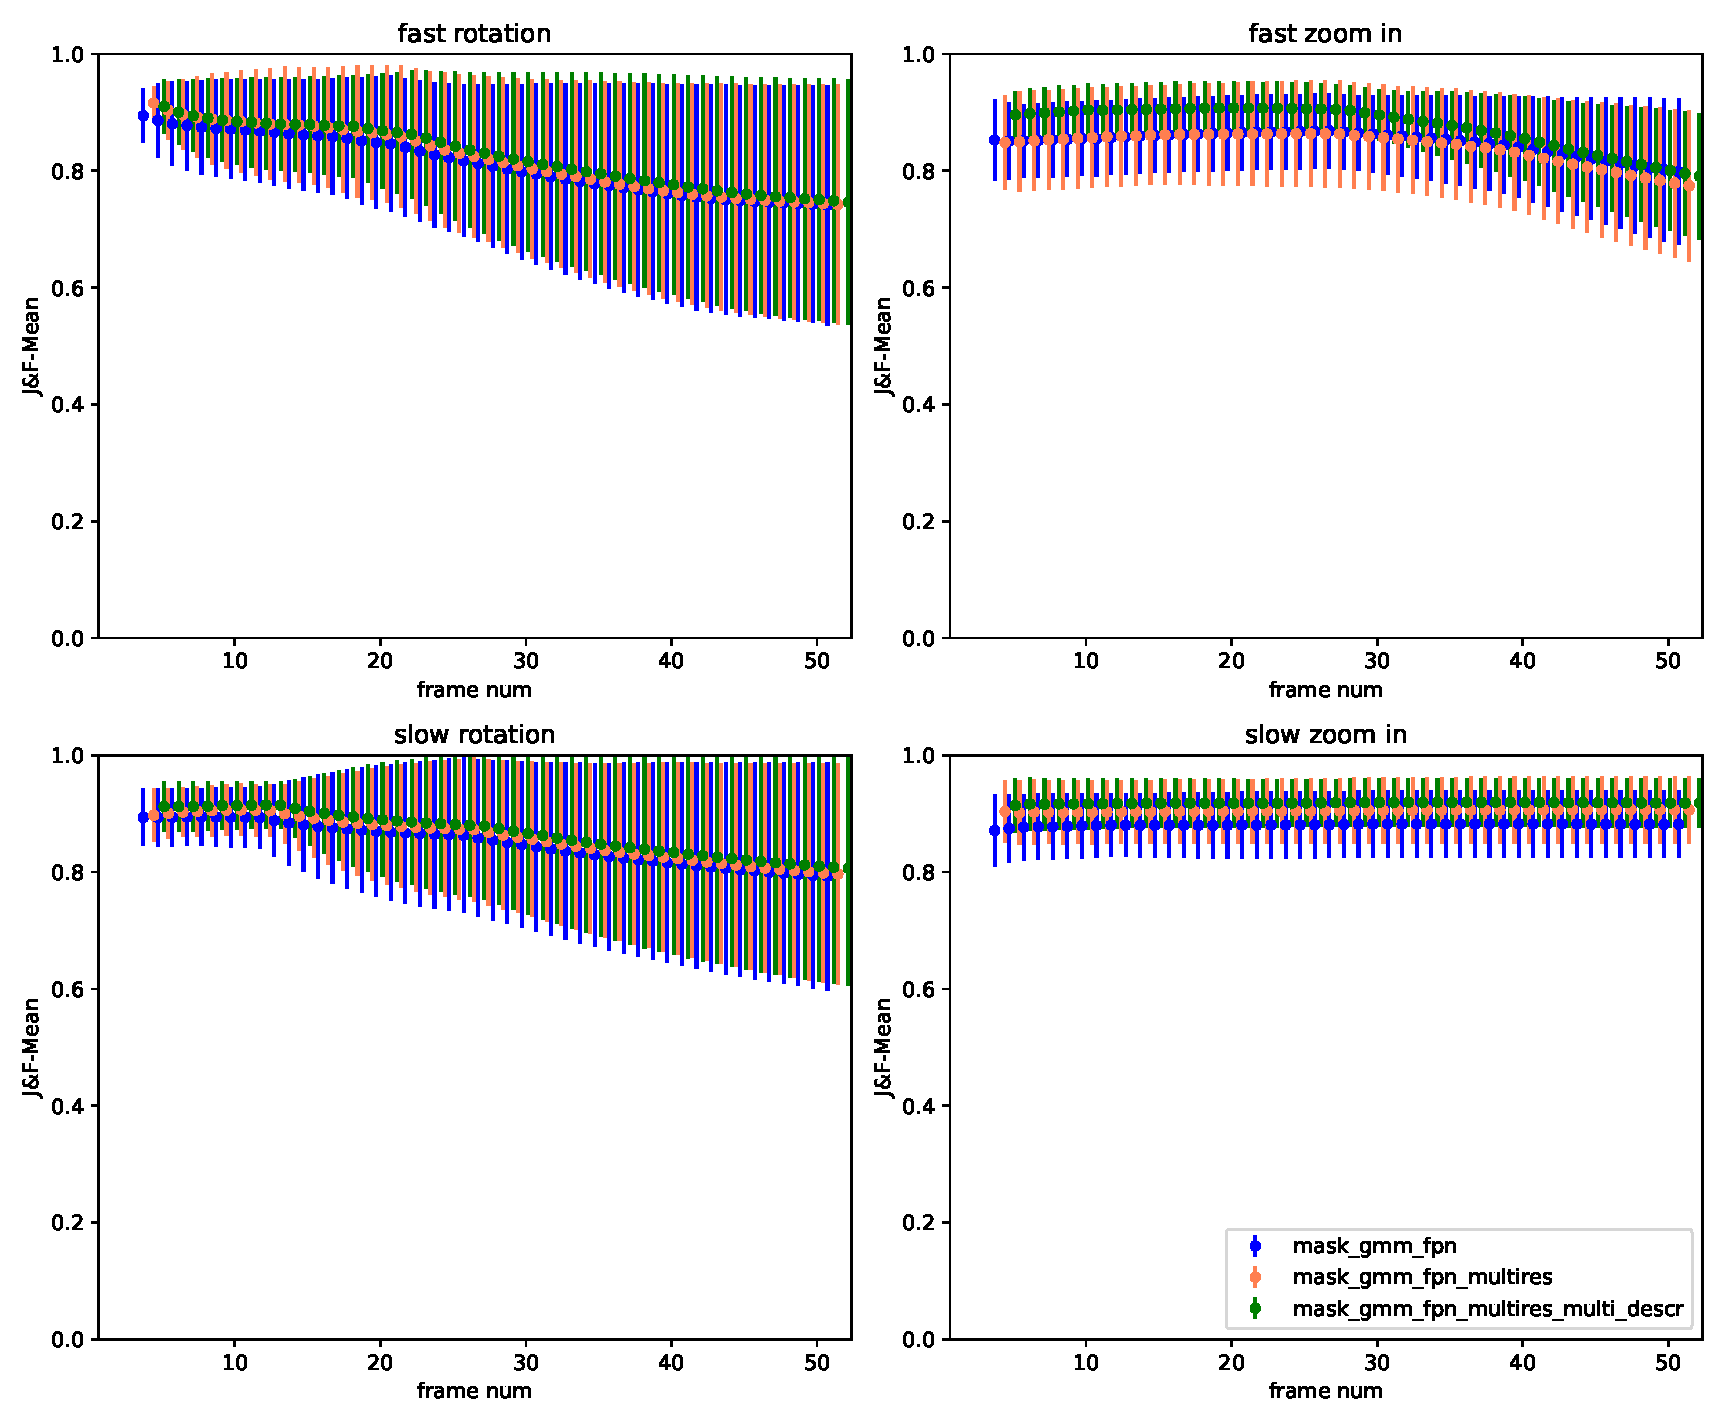
\includegraphics[width=1.\linewidth]{figures/04_experiments/multires_comparisons/mask_gmm_fpn-mask_gmm_fpn_multires-mask_gmm_fpn_multires_multi_descr-movement_all_variance.pdf}
    \caption{Temporal analysis of single- vs multi-scale matching variants (with \\ variance)}
    \label{fig:multires_abl_all_multires}
    
\end{figure}
Observing the preliminary results on the our own test set, the multi-scale model variant with multiple background descriptors presents superior performance to all other model variants. Also in the temporal domain, we note that the multi-scale multi-background model retains a higher $J\&F$ score for more frames in the challenging fast zoom in group compared to the rest of model alternatives. Cross domain, on DAVIS, the multi-scale multi-background model variant also presents a notable performance gap to the other options, which seems to confirm our hypothesis that multiple descriptors for the background result in more refined foreground/ background separation even in completely unknown setups. Naturally, the proposed multi scale multi background solution comes with the drawback of longer inference time, so in some cases it may not be preferred to other faster alternatives. However, as already mentioned, further optimisation in terms of resource allocation for the GMM matchers is possible, but is left as future work. \par

Another interesting observation from this analysis is related to multi-scale vs single-scale matching in the standard case with a single descriptor for both the background and the objects. From the data, it appears that the gain from just expanding the matching strategy to multi scale without multiple background descriptors is negligible, if not non existent. This finding agrees also with the little benefit observed when using the multi scale FPN decoder instead of the MLP decoder in the decoder section comparison. \par

At the end of this section, comparing all possible model variants, the best performance is achieved with the multi scale multi background mask encoder, GMM matching and an FPN decoder. This model variant achieves  a 0,762 $J\&F$ score on our test set and is used as our proposed method version, referred to as GMMTrack in the following section. Next, GMMTrack is compared with a baseline method and tracker. Furthermore, a qualitative analysis is performed on real life data, to provide an intuition about the magnitude of the sim2real gap resulting from training on a synthetic dataset but testing on real RGB stereo input data. 

%here you 'll add a table with everything
\section{Final evaluation and experiments}
\subsection{Comparison with single shot segmentor}

The first comparison of the proposed method with a baseline is with the single shot instance segmentation method INSTR \parencite{durner2021unknown}. INSTR, like any single shot segmentation algorithm, can be converted to a naive heuristic tracker by adding a matching/association step with the previous frame prediction. In this work, INSTR is converted to a heuristic based tracker with IoU association. Details on INSTR+IoU are provided in \autoref{subseq:instr}.\par
In general, the performance of association-based trackers is strongly dependent on the segmentation quality achieved by the neural network they build upon \parencite{sort}. Hence, before converting INSTR into a baseline tracker, we ensure that the single shot segmentation performance on our test set achieves a high volumetric mIoU score, if all frames in all sequences are treated as individual test inputs. Indeed, INSTR achieves a 0,774 mIoU on our test set and is expected to perform adequately well as a tracker with IoU association. \par

A qualitative overview of single shot segmentation with INSTR on a test set sequence, treating each frame individually, is provided in \figref\ref{fig:qualitative_instr}. For visualisation purposes, both in \figref\ref{fig:qualitative_instr_sketo} and the ones that follow predictions are visualised every 5 frames in a 10 frame grid for a 50 frame sequence. For 100 frame long sequences, encountered in later experiments, predictions are included in the grid visualisation every 10 frames. \par



\begin{table} [ht!]
\caption{Comparison with single shot segmentation network INSTR}
\centering

\begin{tabular}{|c|c|c|c|c|} 
\hline
Model    & vol. mIoU & J &  F & J\&F\\ 
\hline

INSTR & 0.774 & - & - & - \\
INSTR + IoU ass. & - & 0.578 &  0.636 & 0.607\\
GMMTrack(ours) & - & 0.722  & 0.802 & 0.762  \\
%GMMTrack(ours) with INSTR init & - &  \\
\hline
\end{tabular}
\end{table}

\begin{figure}[!ht]
    \subfloat[Inference on scene 4 rotation fast with INSTR\label{fig:qualitative_instr_sketo}]{%
      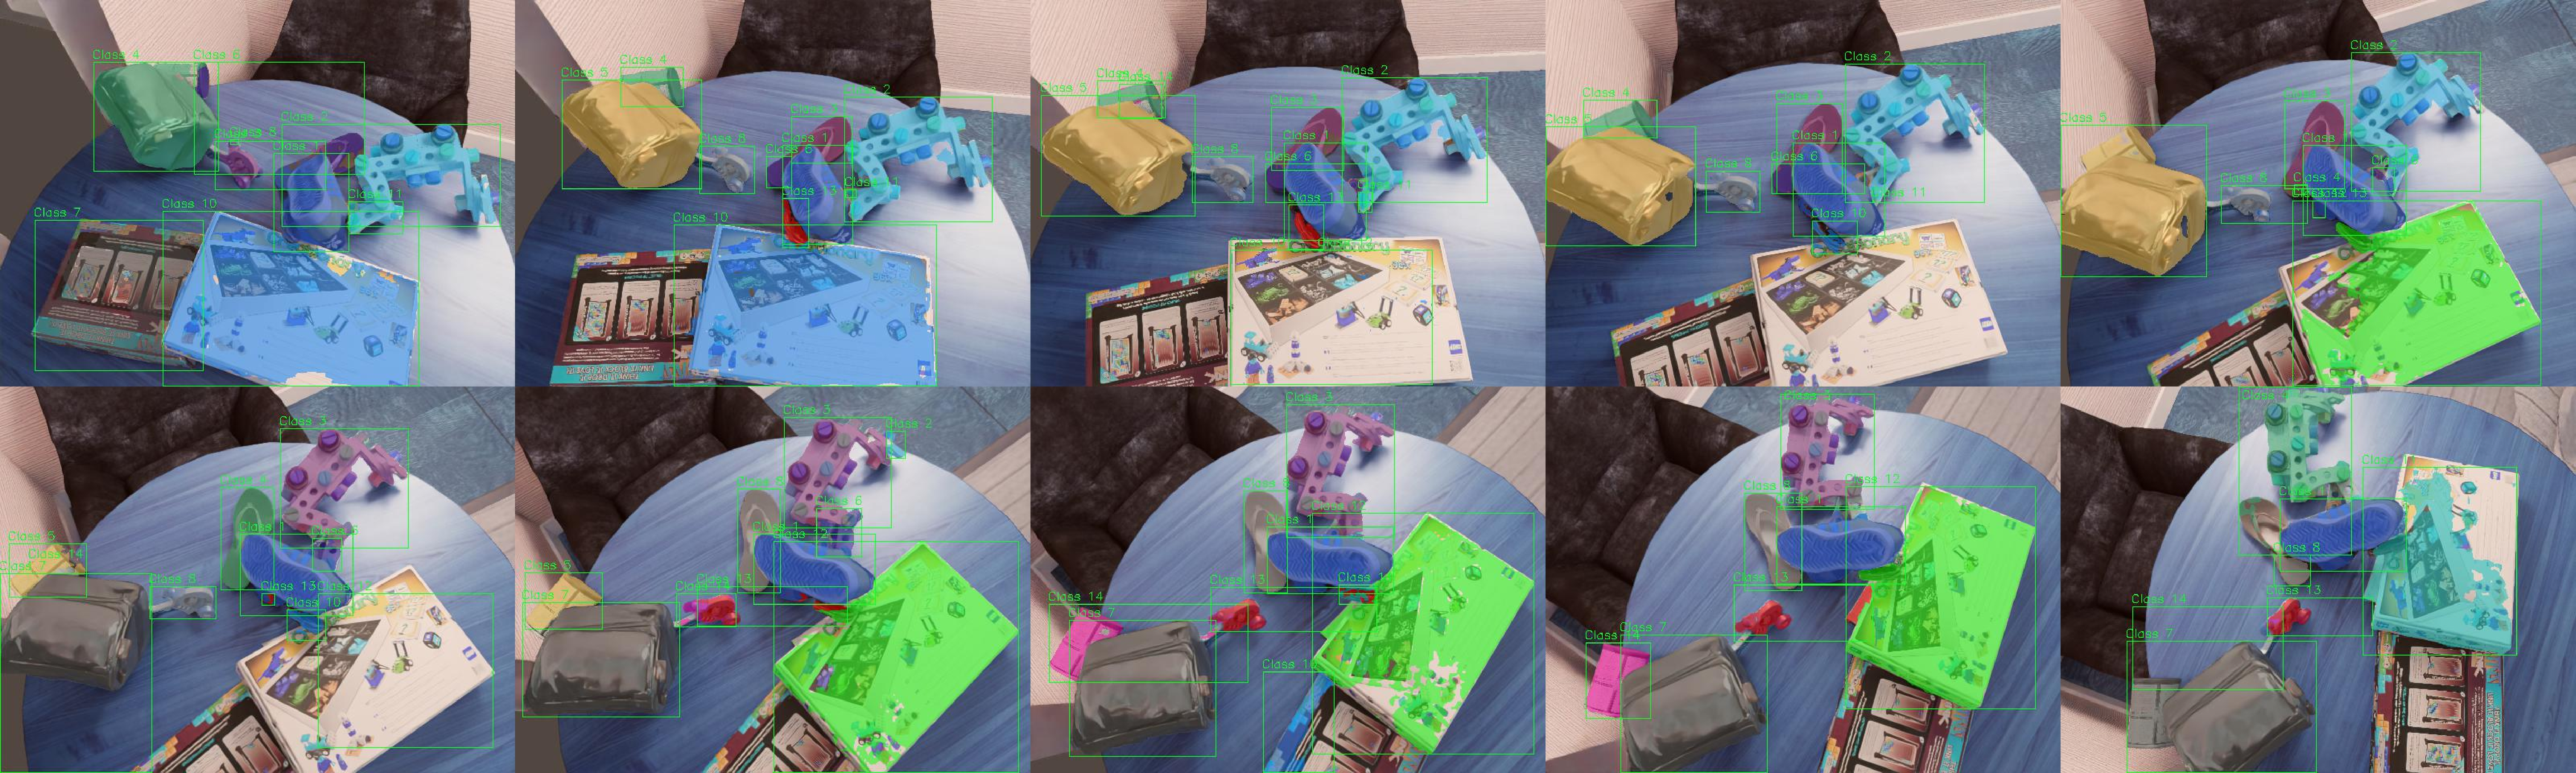
\includegraphics[width=1.\linewidth]{figures/qualitative_instr/instr_overlays.pdf}
    }
    \hfill
    \subfloat[Inference on scene 4 rotation fast with INSTR+IoU\label{fig:qualitative_instr_iou}]{%
      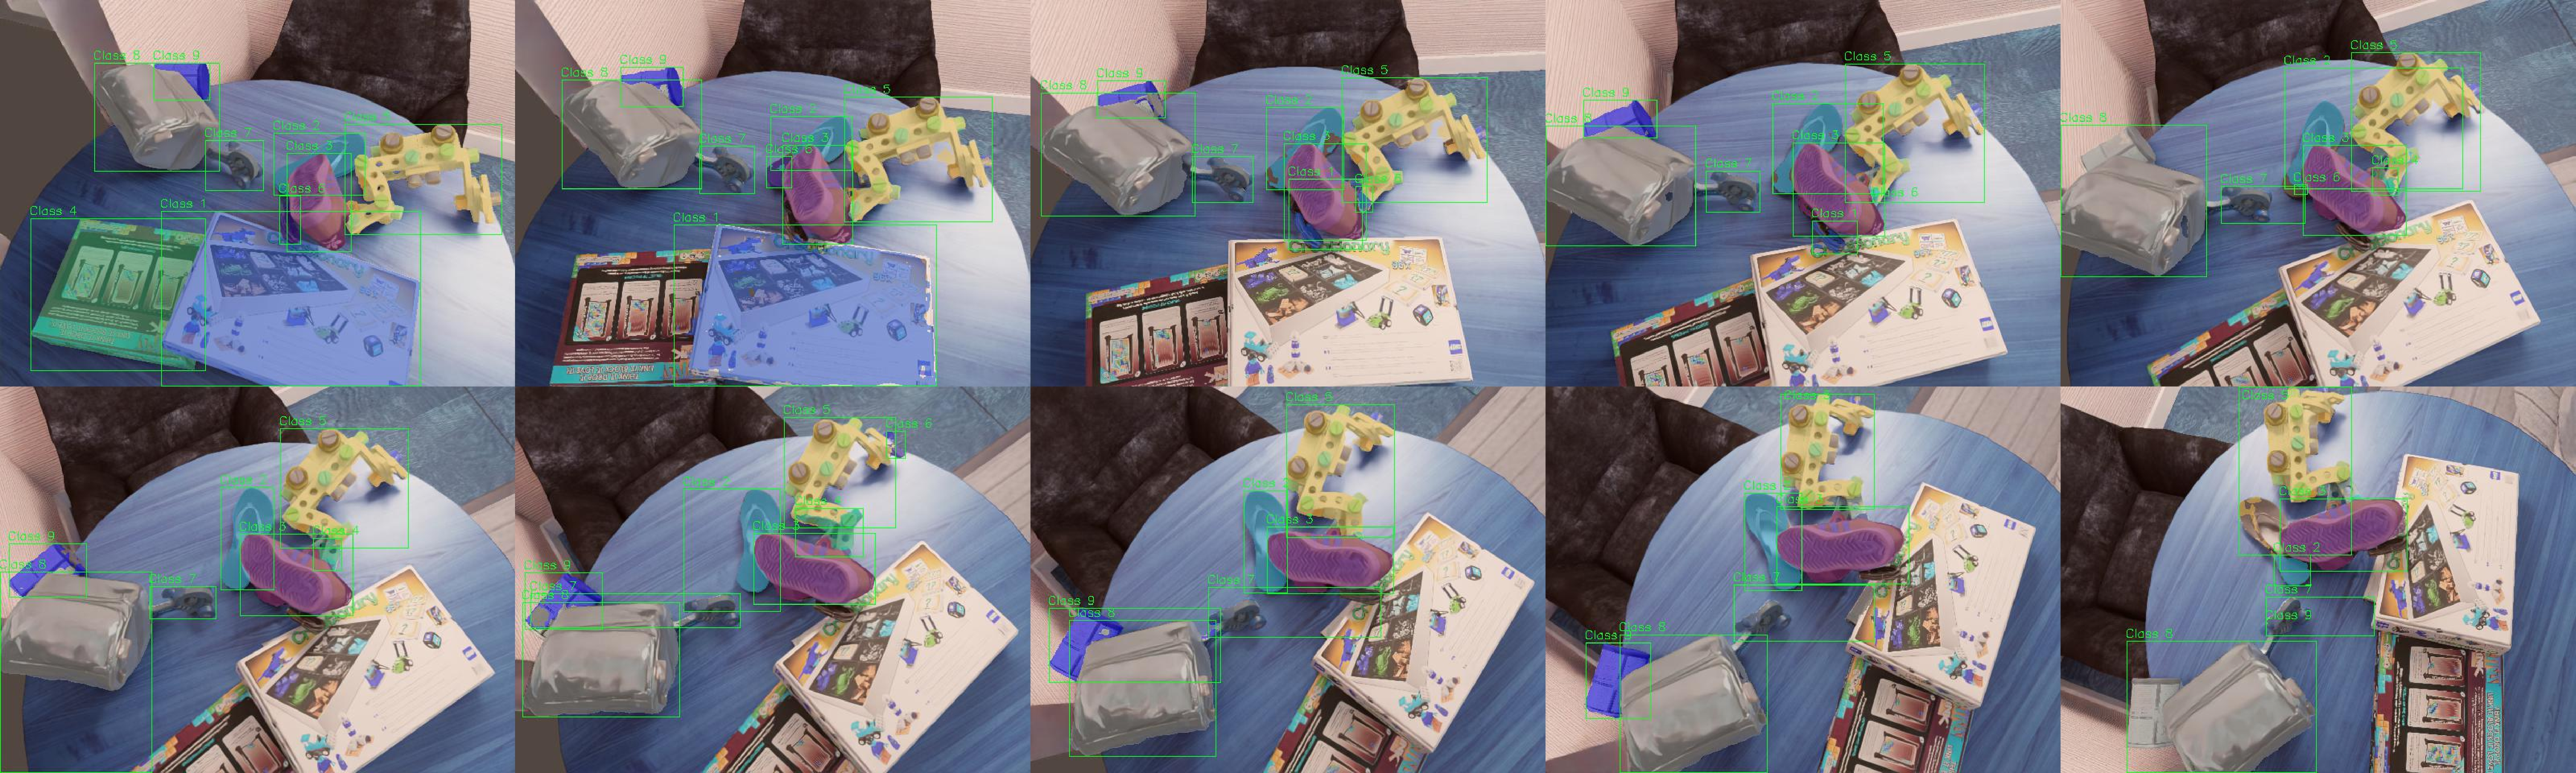
\includegraphics[width=1.\linewidth]{figures/qualitative_instr/instr_iou_overlays.pdf}
    }
    \hfill
    \subfloat[Inference on scene 4 rotation fast with GMMTrack\label{fig:qualitative_instr_gmm}]{%
      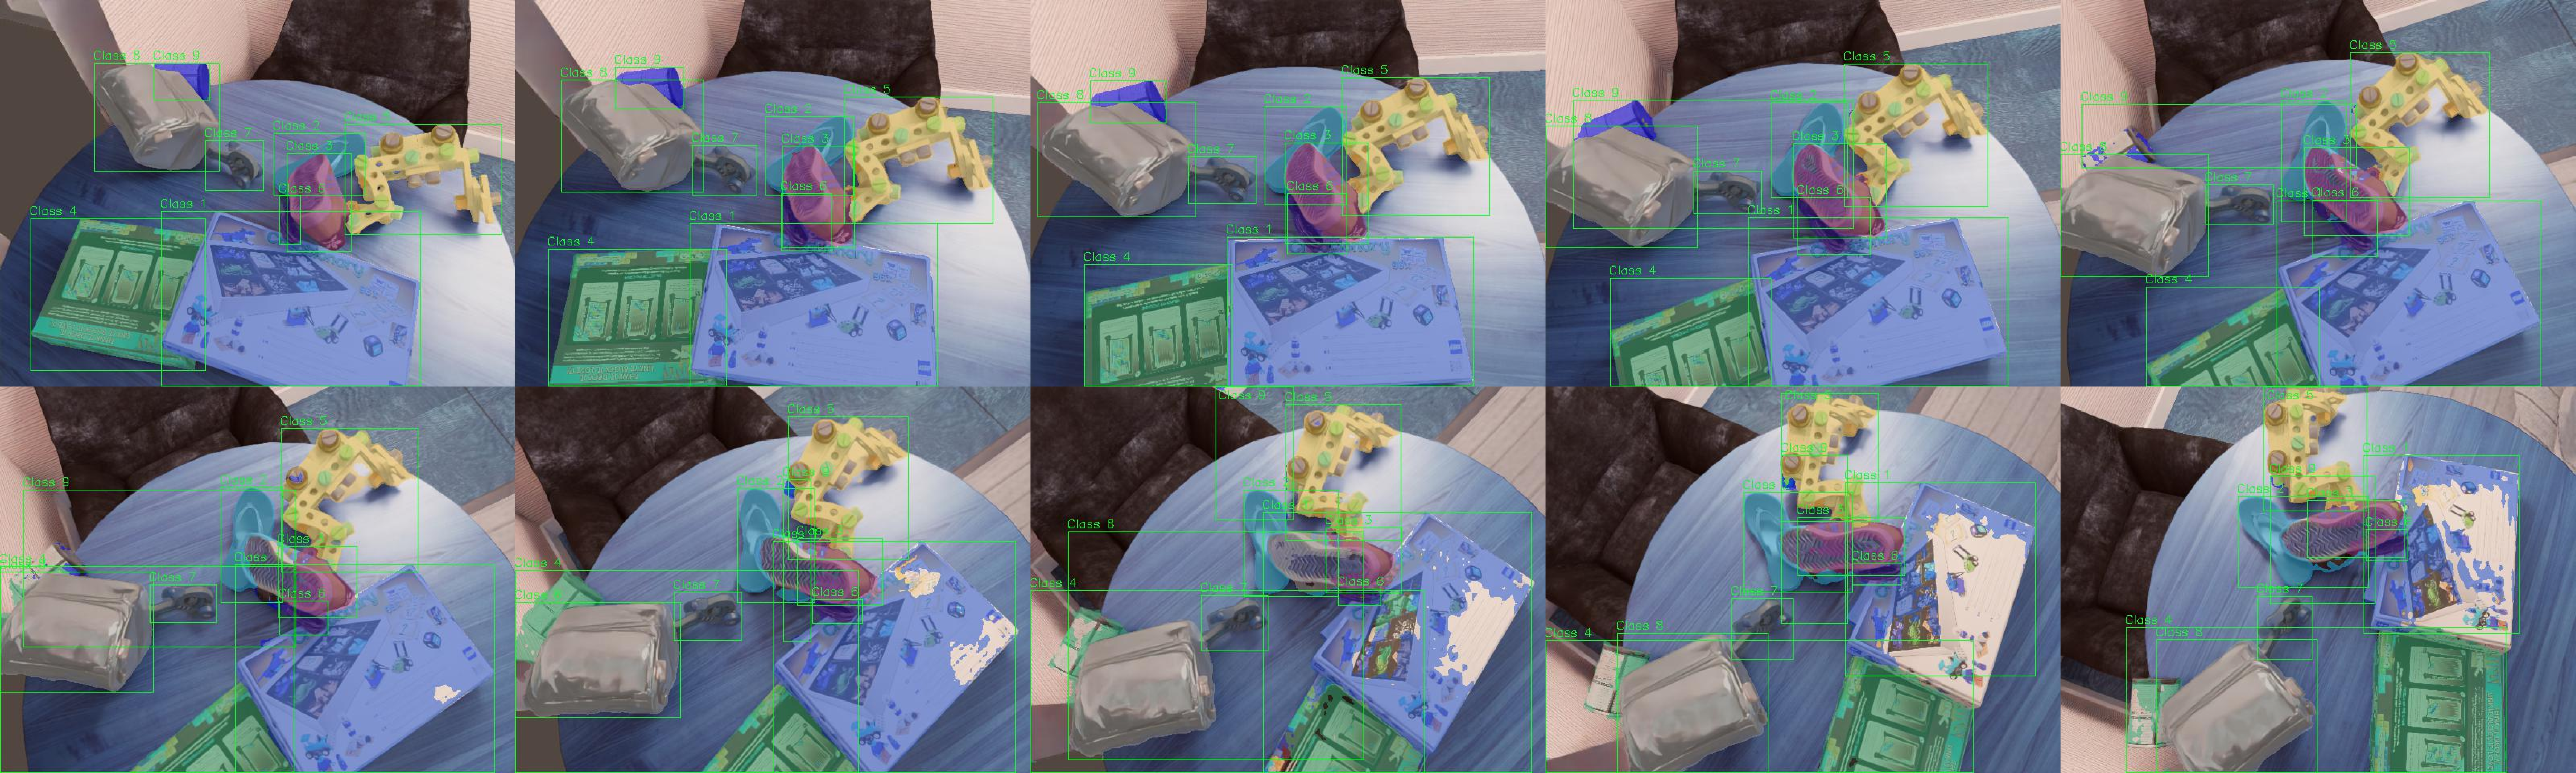
\includegraphics[width=1.\linewidth]{figures/qualitative_instr/mask_gmm_fpn_overlays.pdf}
      }
    \caption{Comparison with single shot segmentation network INSTR 
    }
    \label{fig:qualitative_instr}
\end{figure}

 
After converting INSTR into a tracker with IoU association, we can assess the method on our tracking test set with the standard $J\&F$ tracking metrics used in the rest of our experiments. We note that the INSTR+IoU association achieves a 0,607 $J\&F$ score, which is lower than the worst performing variants of the proposed method, like the bounding box based encoder or the responsibilty upsampler with a mask encoder and GMM matching. However, this is expected, as heuristic-based trackers do not integrate past frame information to improve their predictions. The predictions result solely from the encodings of the current frame and are only assigned a temporally consistent track id by association with the previous frame prediction. If the network fails to detect an object in the current frame, due to occlusions or some other difficulty in the scene, the past frame encodings are not available to potentially guide the network to a more informed prediction, like in the case of learning-based trackers with some matching mechanism. Moreover, in case of dramatic appearance changes or non negligible displacement of an object between frames, the >0.5 IoU threshold is typically not satisfied and id assignment based on the IoU overlap does not result in correct id propagation for the same object in different frames.  \par

A qualitative comparison between INSTR+IoU and GMMTrack in a difficult scene for INSTR+IoU is presented in \figref\ref{fig:qualitative_instr_iou} and \figref\ref{fig:qualitative_instr_gmm}. As time progresses, IoU association fails for some classes and they are not included in the predicted binary masks. Common source of such prediction errors is oversegmentation or mask leaking in the estimated masks for the current frame. This faulty mask prediction results in failure of association with the predicted mask from the previous frame and initiates a spiral of error propagation in the sequence.


\subsection{Comparison with SOTA}
%you can get the numbers on DAVIS directly from the paper if they have them for the checkpoint you used. Otherwise setup davis inference from checkpoint! with temporal analysis and all! 


HODOR is compared to our method in two ways. Firstly, the pretrained model on static images is used out of the box on our test data. Secondly, the static images checkpoint is finetuned on our synthetic tracking dataset for 120000 iterations based on the provided recipe for training on sparsely annotated videos \parencite{HODORgithub}. Observing the achieved performance, it appears that finetuning on our dataset does not improve the performance obtained with the static image checkpoint. Evidently, the large scale training on COCO with image augmentations as past frames suffices in order for HODOR to achieve good performance on our test set and no new knowledge is added to the model via finetuning. To the contrary, the model seems to be led to overfitting, which is also reported by  \cite{athar2022hodor} in some of their attempts to finetune on sparse video. In total, HODOR achieves similar performance to our proposed tracking method, probably due to the more sophisticated but computationally costly past information encoding mechanism with an additional self-attention mechanism and the elaborate masked attention on matching. \par 



%TODO: add more detailes about checkpoint and our training 
 

\begin{table}[ht!]
\caption{Comparison with SOTA semi-supervised tracker HODOR}
\centering
\begin{tabular}{|c|ccc|}
\hline
\multicolumn{1}{|c|}{\multirow{2}{*}{Decoder Type}} & \multicolumn{3}{c|}{Tracking Dataset}                                                                                                   \\ \cline{2-4} 
\multicolumn{1}{|c|}{}                              & \multicolumn{1}{c|}{J} & \multicolumn{1}{c|}{F} & \multicolumn{1}{c|}{J\&F} \\ \hline

GMMTrack (ours)   & 0.722  & 0.802 & 0.762 \\  %\cline{1-1}
HODOR         & 0.720  & 0.790  & 0.755  \\ %\cline{1-1}

HODOR finetuned   & 0.718   & 0.777  & 0.747  \\ \hline

\end{tabular}
\end{table}

Qualitatively, HODOR predicts accurate masks both in terms of region similarity and contour accuracy, as can be seen in \figref\ref{fig:qualitative_hodor}. However, HODOR in all its variants completely ignores small objects, as in the case of class 5 in scene 1 of our synthetic dataset, see \figref\ref{fig:qualitative_hodor}. For comparison, the predictions with our model are visualised every 5 frames in \figref\ref{fig:qualitative_mask_gmm}. It is evident that our method predicts all classes regardless of the annotation size, including class 5 with a very small annotation in frame 0. This behaviour of HODOR is expected, since small objects are filtered out during initialisation and excluded from training. This might be one of the reasons why even after fine tuning on our training set, HODOR does not improve much in performance. Indeed, regardless of the accuracy achieved on a region similarity or contour level, completely ignoring classes in the predictions is heavily penalised by the $J\&F$ metric.\par 


\begin{figure}[!ht]
    \subfloat[Inference on scene 1 rotation slow with GMMTrack\label{fig:qualitative_mask_gmm}]{%
      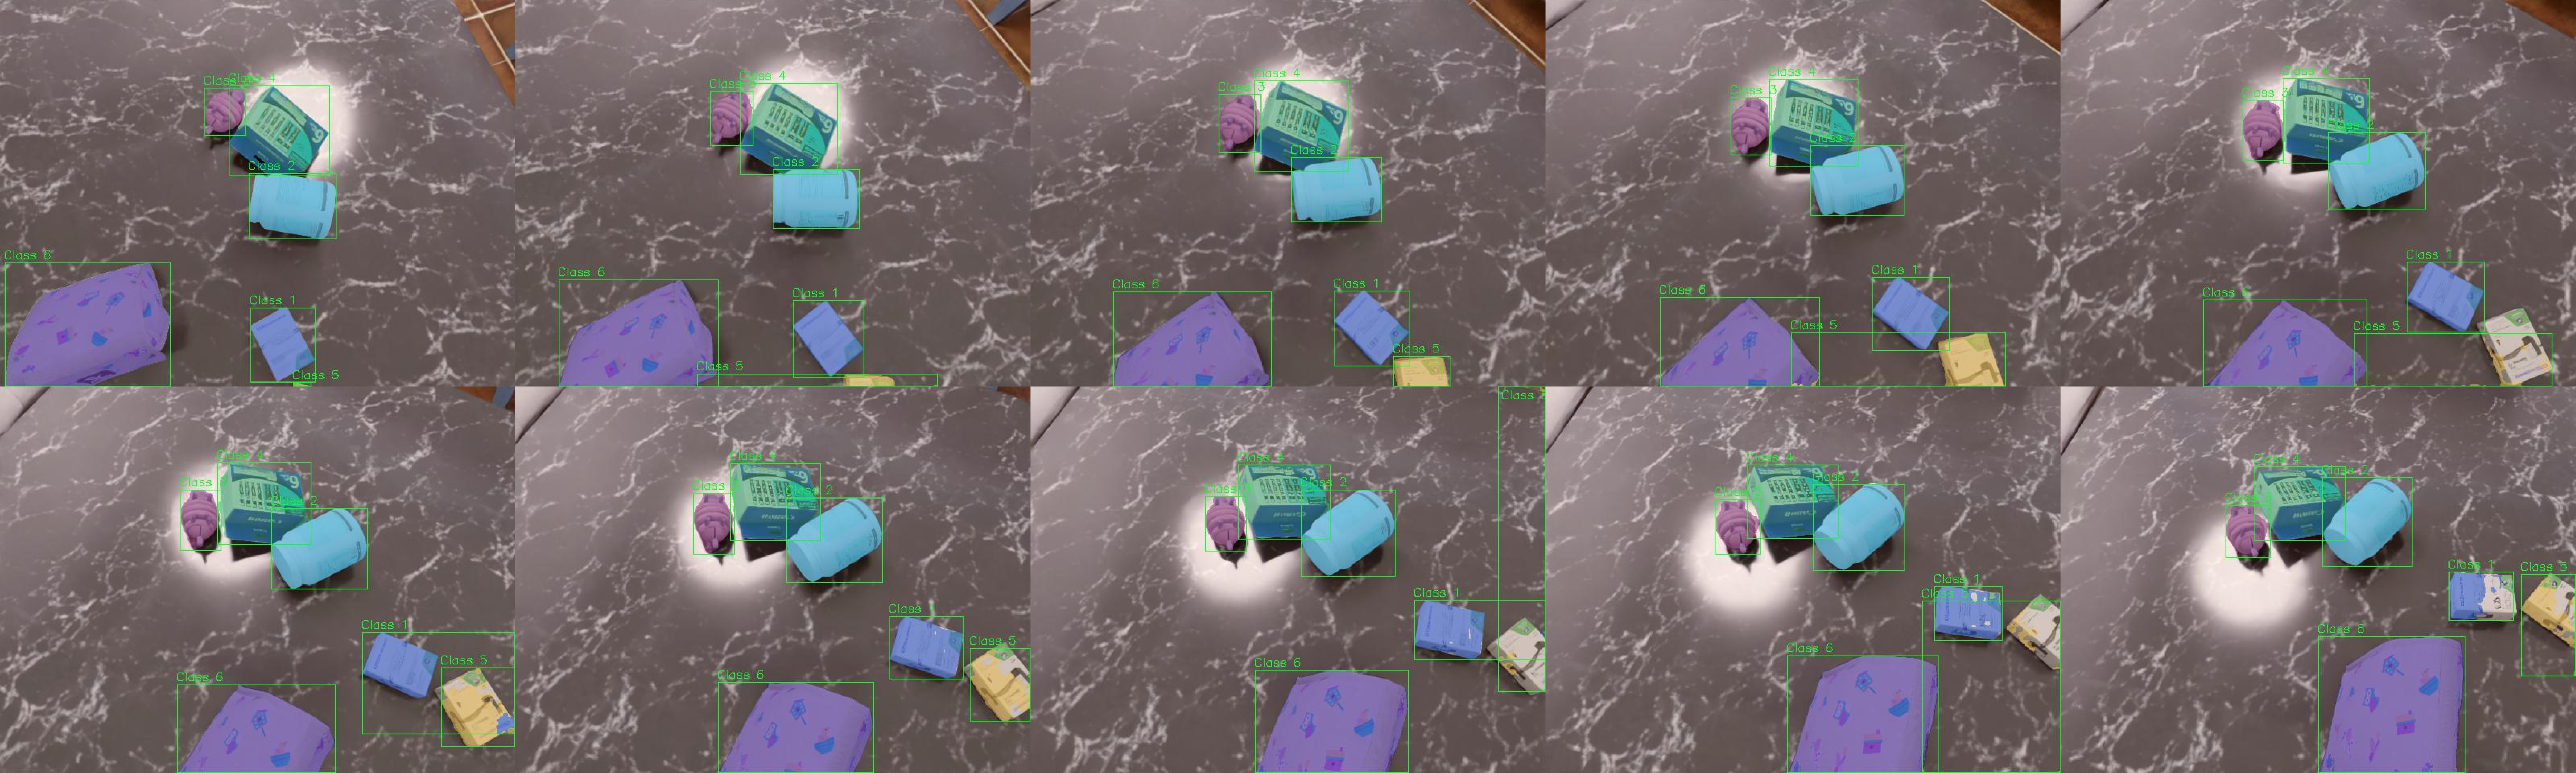
\includegraphics[width=1.\linewidth]{figures/qualitative_comparison_hodor/mask_gmm_overlays.pdf}
    }
    \hfill
    \subfloat[Inference on scene 1 rotation slow with HODOR\label{fig:qualitative_hodor}]{%
      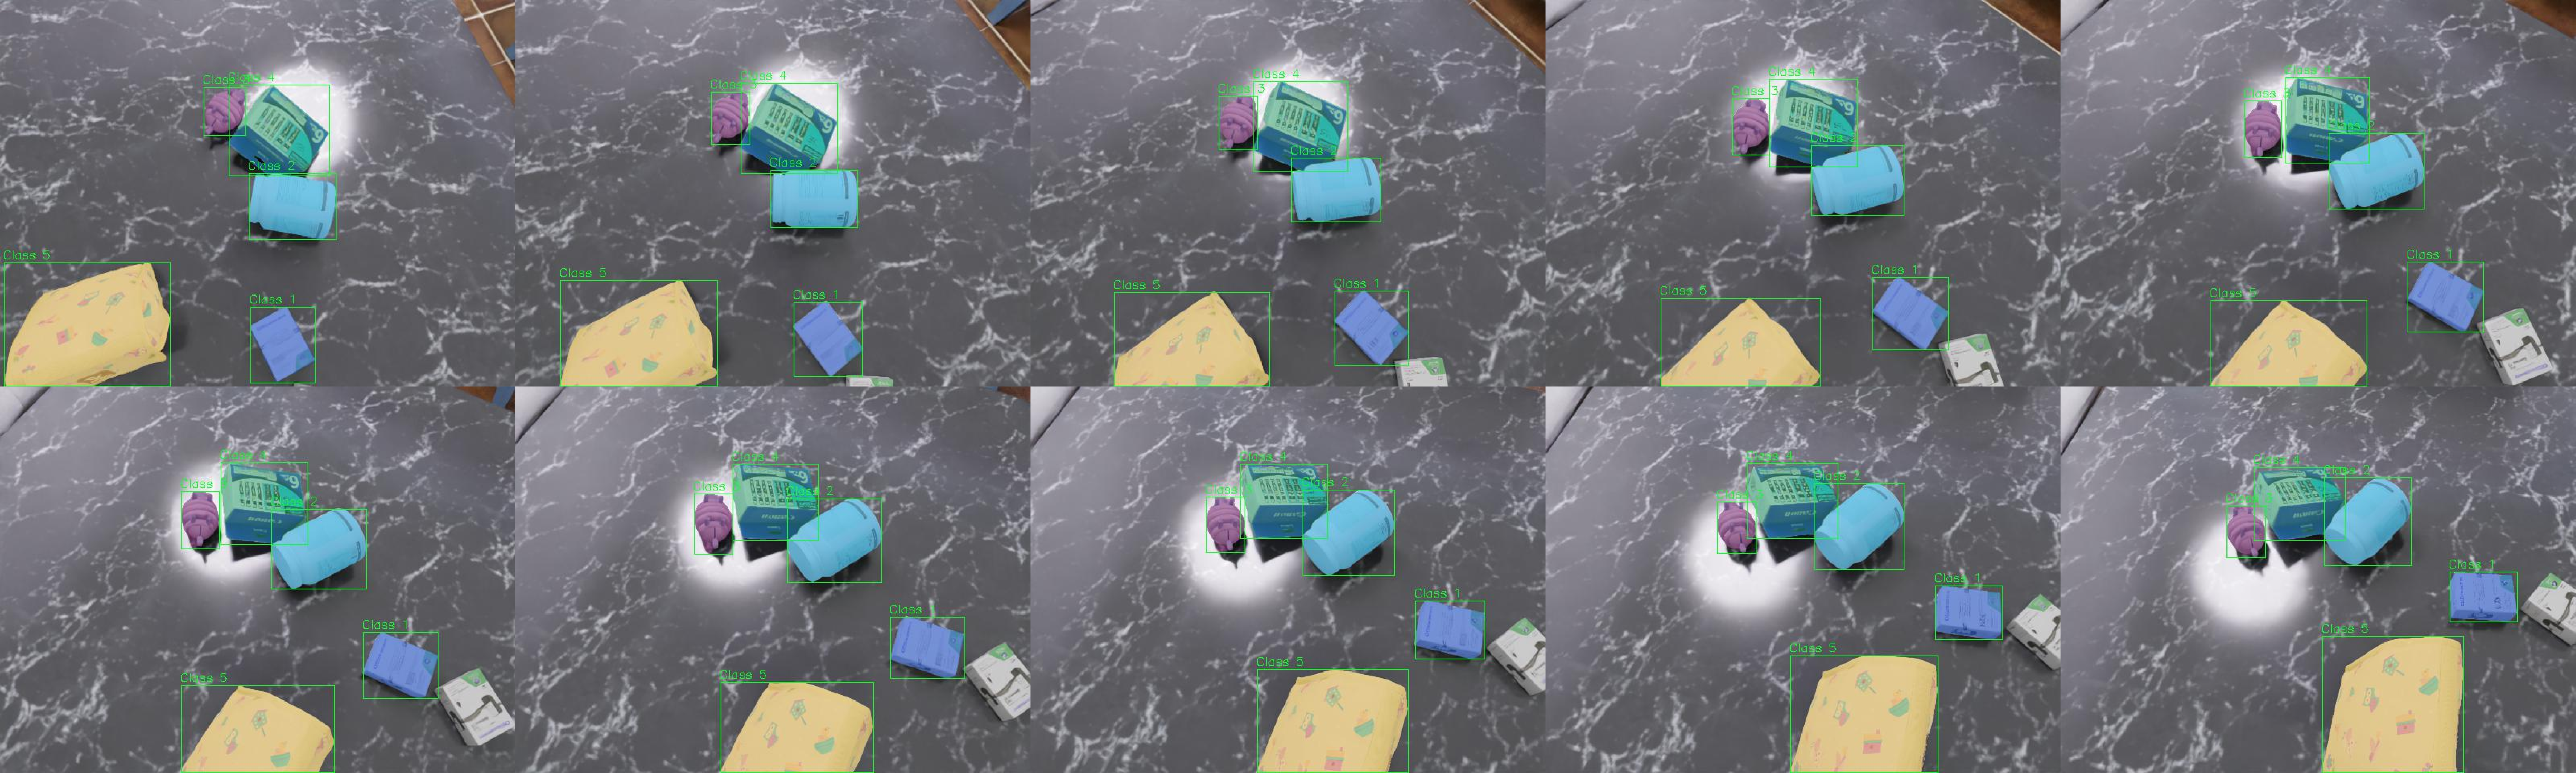
\includegraphics[width=1.\linewidth]{figures/qualitative_comparison_hodor/hodor_overlays.pdf}
    }
    \caption{Comparison with semi-supervised tracker HODOR
    }
    \label{fig:qualitative_hodor_all}
\end{figure}



\subsection{Qualitative analysis on real data}
%here you 'll add a table with everything

Apart from the quantitative analysis presented in the previous sections, a qualitative analysis on real data was performed to provide an intuition on the sim2real gap for our method after training on a synthetic dataset. Ideally, this analysis would have taken place quantitatively. However, creating a real life annotated test set, with sequences recorded during real robotic manipulations, exceeds the scope of this thesis. \par
\newpage
Without having access to annotations, initialising our method is slightly more challenging. In practice, GMMTrack is initialised with predictions provided by the single shot segmentation network INSTR for the purpose of this analysis. In theory, this initialisation can also happen with a human in the loop in a real life scenario, and this is also an interesting direction left as future work. \par

The GMMTrack predictions with INSTR initialisation are compared with single shot INSTR predictions (without tracking) in two setups. In the first scene, the objects are scattered in front of a relatively neutral background, with distance between them. Even though some furniture parts are visible in the back of the frames, they are not included in the predicted segmentation masks, neither by GMMTrack see \figref\ref{fig:qualitative_floor_GMMTrack} nor by INSTR see \figref\ref{fig:qualitative_floor_instr}. The only difference between the two networks is that GMMTrack, as expected, predicts temporally consistent masks, since it assigns the same class for the same object in the whole sequence. This is not the case for INSTR, though in this easy scene, just adding the IoU association step would most probably be enough to correctly assign the ids throughout the frames, since the objects change only slightly in scale and appearance in the course of the sequence. \par

\begin{figure}[!ht]
    \subfloat[Inference on floor sequence with INSTR\label{fig:qualitative_floor_instr}]{%
      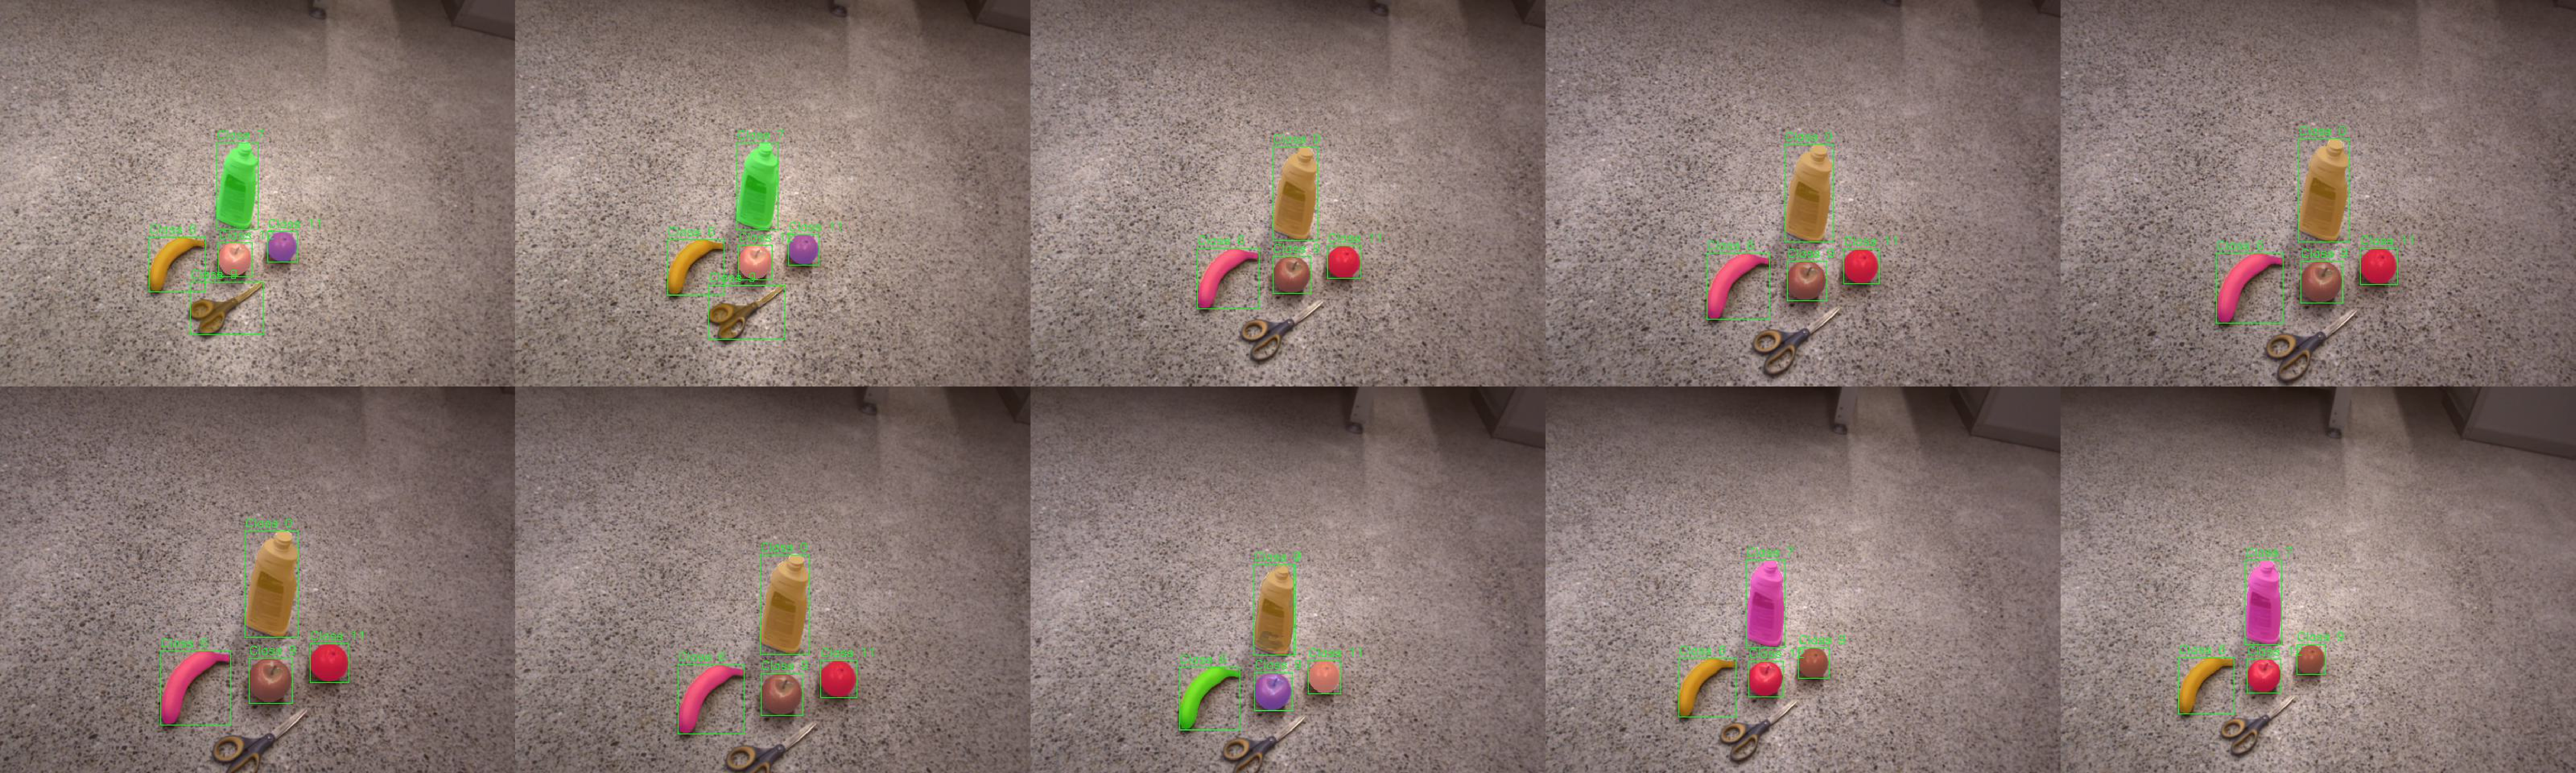
\includegraphics[width=1.\linewidth]{figures/qualitative_analysis_stereo/zoom_in_out_5_objs_overlays_instr.pdf}
    }
    \hfill
    \subfloat[Inference on floor sequence with GMMTrack\label{fig:qualitative_floor_GMMTrack}]{%
      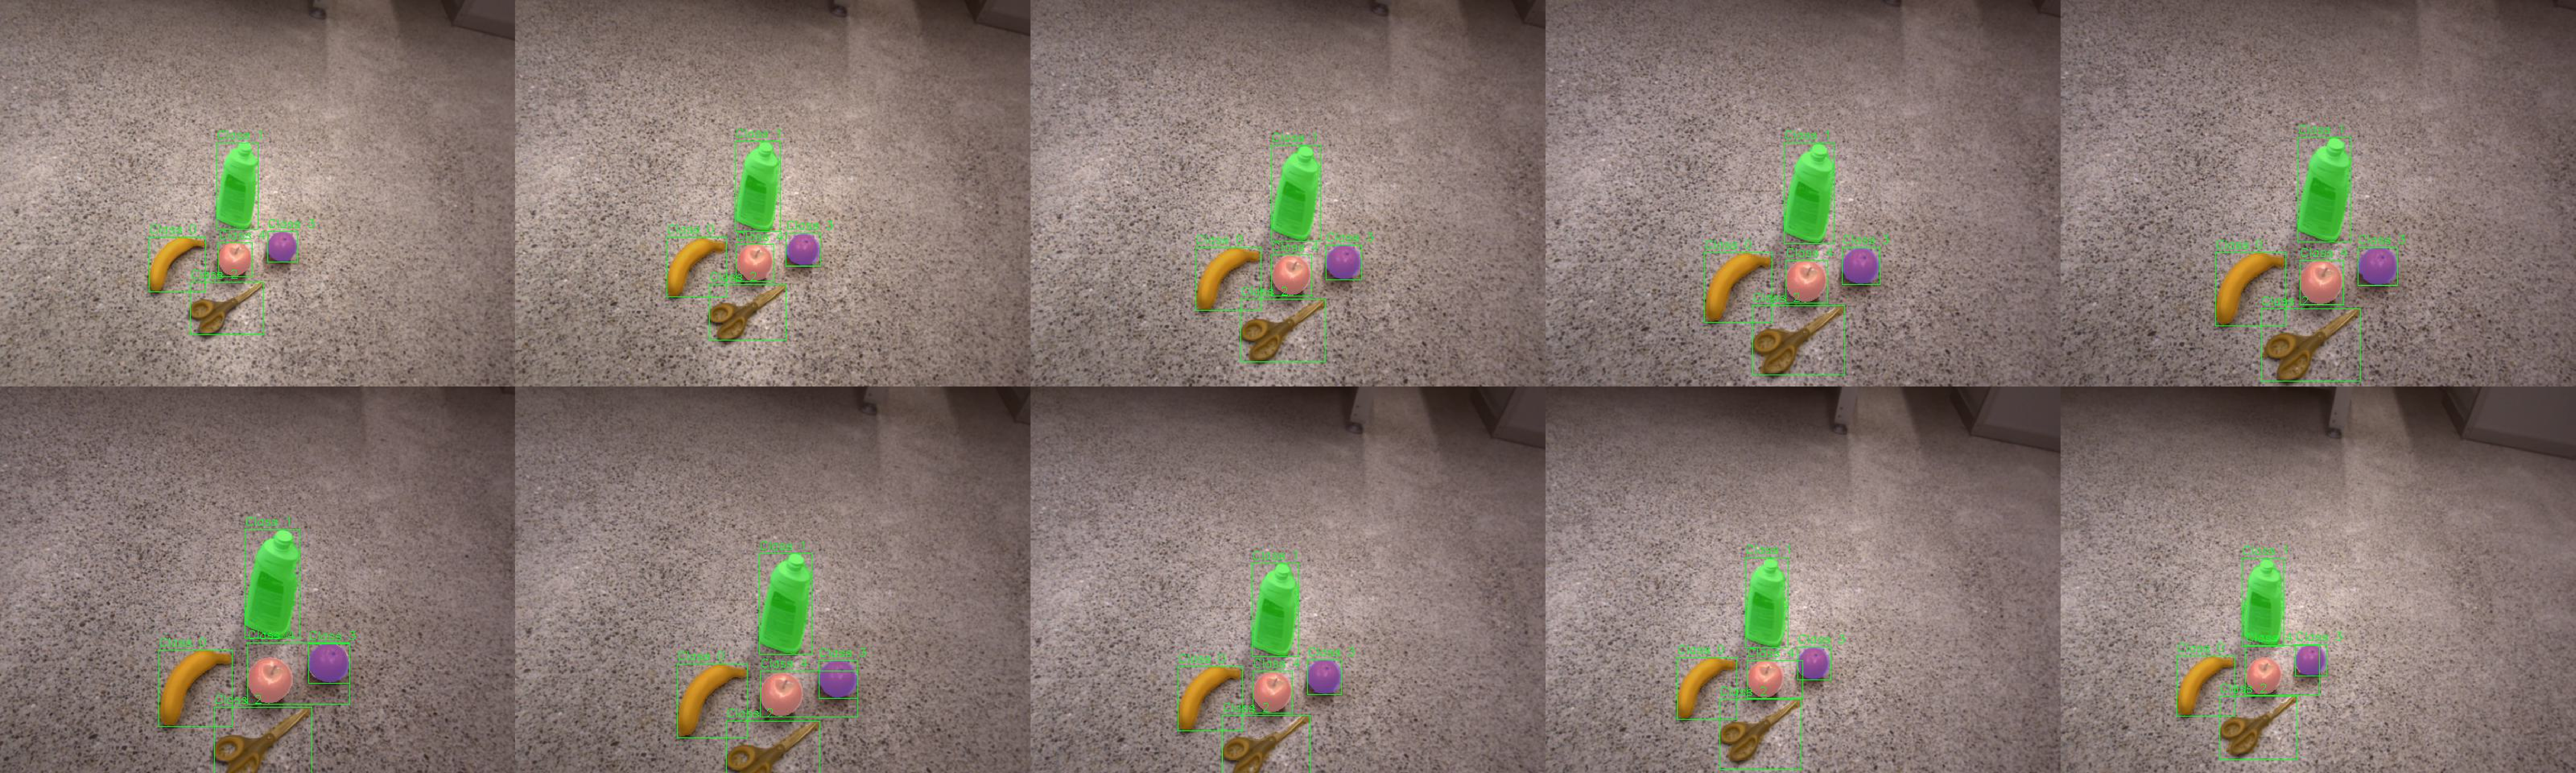
\includegraphics[width=1.\linewidth]{figures/qualitative_analysis_stereo/zoom_in_out_5_objs_overlays_onseg.pdf}
    }
    \caption{Inference on floor sequence 
    }
    \label{fig:qualitative_floor}
\end{figure}

The second scene included in the analysis is shot on the conveyor belt of the robotic lab and is far more challenging than the floor scene. The camera movement is more abrupt and results in dramatic occlusions and reappearances of some objects. Additionally, more background clutter is present in the scene, as various sockets and cables from the lab equipment are visible. Here, it becomes evident how important correct initialisation is for GMMTrack's prediction quality on the sequence. If the network is initialised with correct segmentation masks like in \figref\ref{fig:qualitative_conveyor_GMMTrack}, the masks are correctly predicted for the first 25 frames (frames are included in the grid every 5 frames). Moreover, after the occluded objects reappear in frame 40, the correct ids are recovered. In comparison, INSTR appears to provide worse segmentation quality in cluttered scenes. By frame 15 in \figref\ref{fig:qualitative_conveyor_instr} the soft-scrub object is no longer detected. On the contrary sockets and background clutter are detected as objects of interest. This scenario seems to validate our original hypothesis that tracking can  also help improve segmentation quality in challenging, real life, cluttered scenes. 
% However, a quantitative analysis on a testset with annotations is necessary to officially confirm this hypothesis. 





\begin{figure}[!ht]
    \subfloat[Inference on conveyor belt sequence with INSTR\label{fig:qualitative_conveyor_instr}]{%
      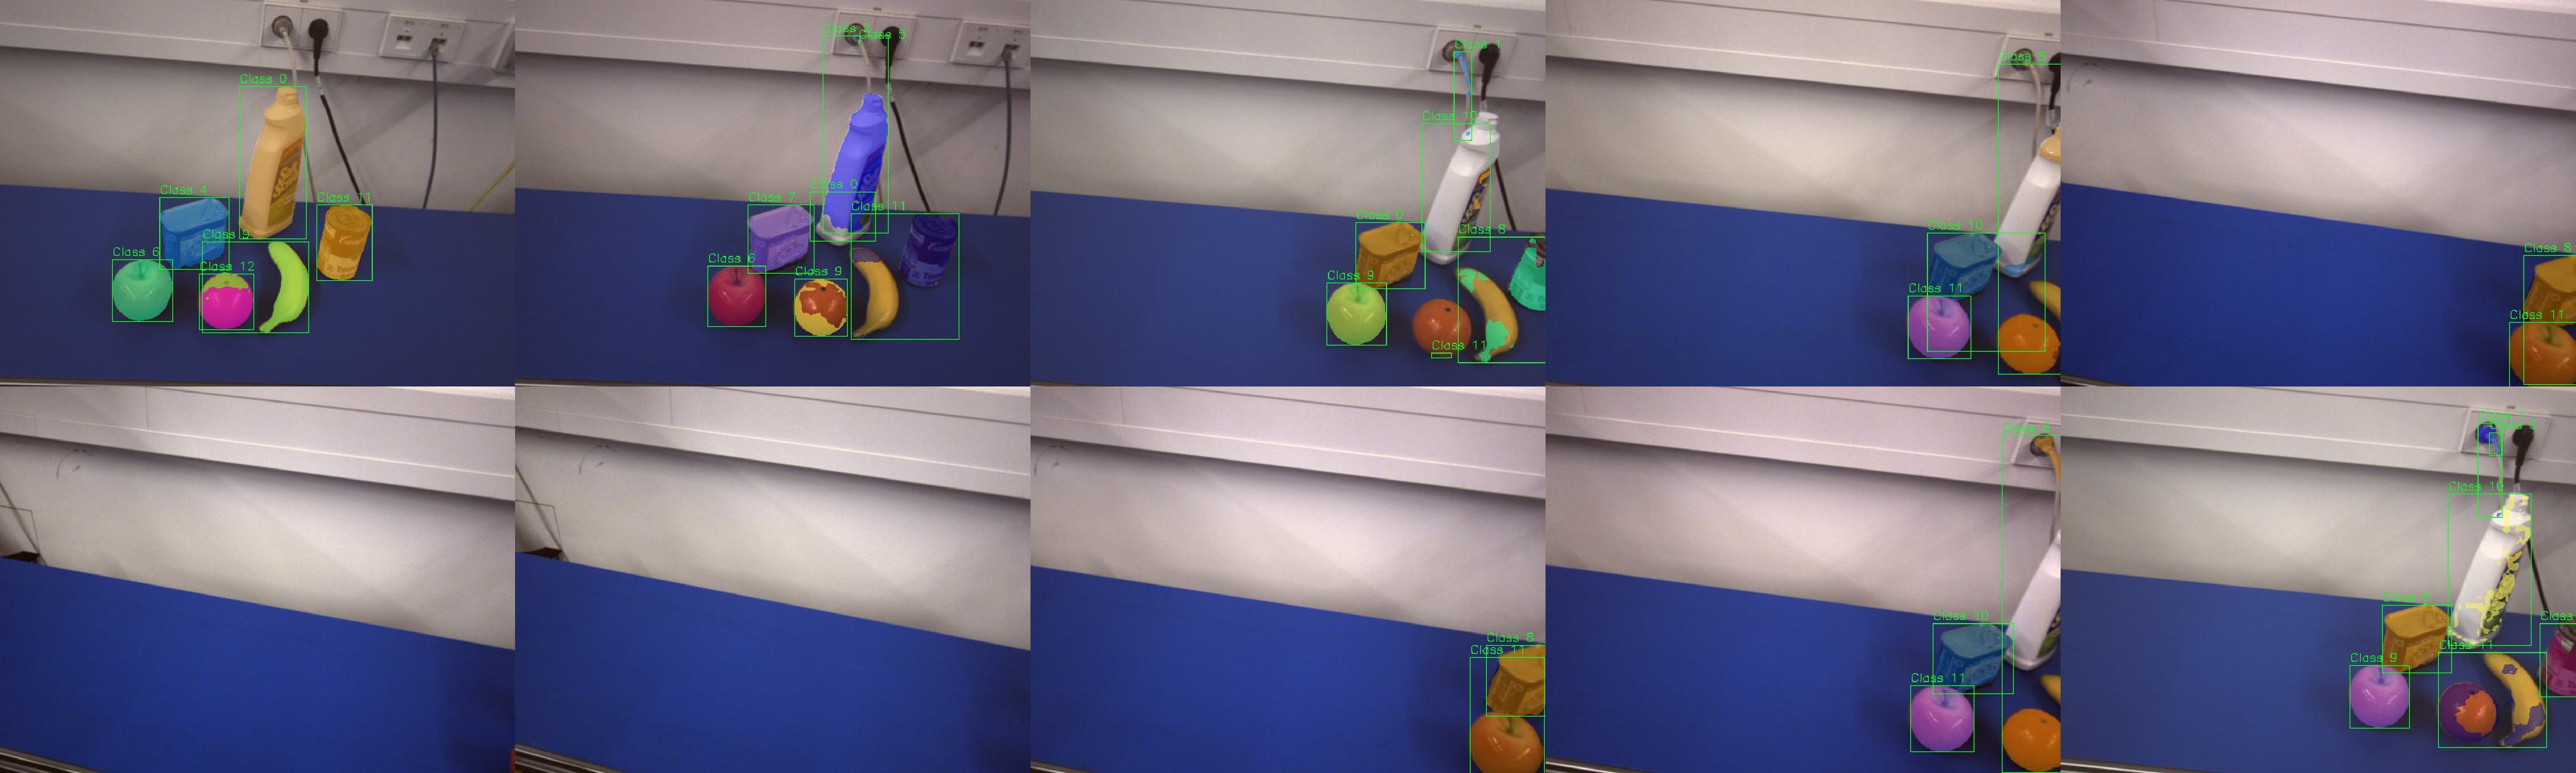
\includegraphics[width=1.\linewidth]{figures/qualitative_analysis_stereo/converer_belt_easy_overlays_instr.pdf}
    }
    \hfill
    \subfloat[Inference on conveyor belt sequence with GMMTrack\label{fig:qualitative_conveyor_GMMTrack}]{%
      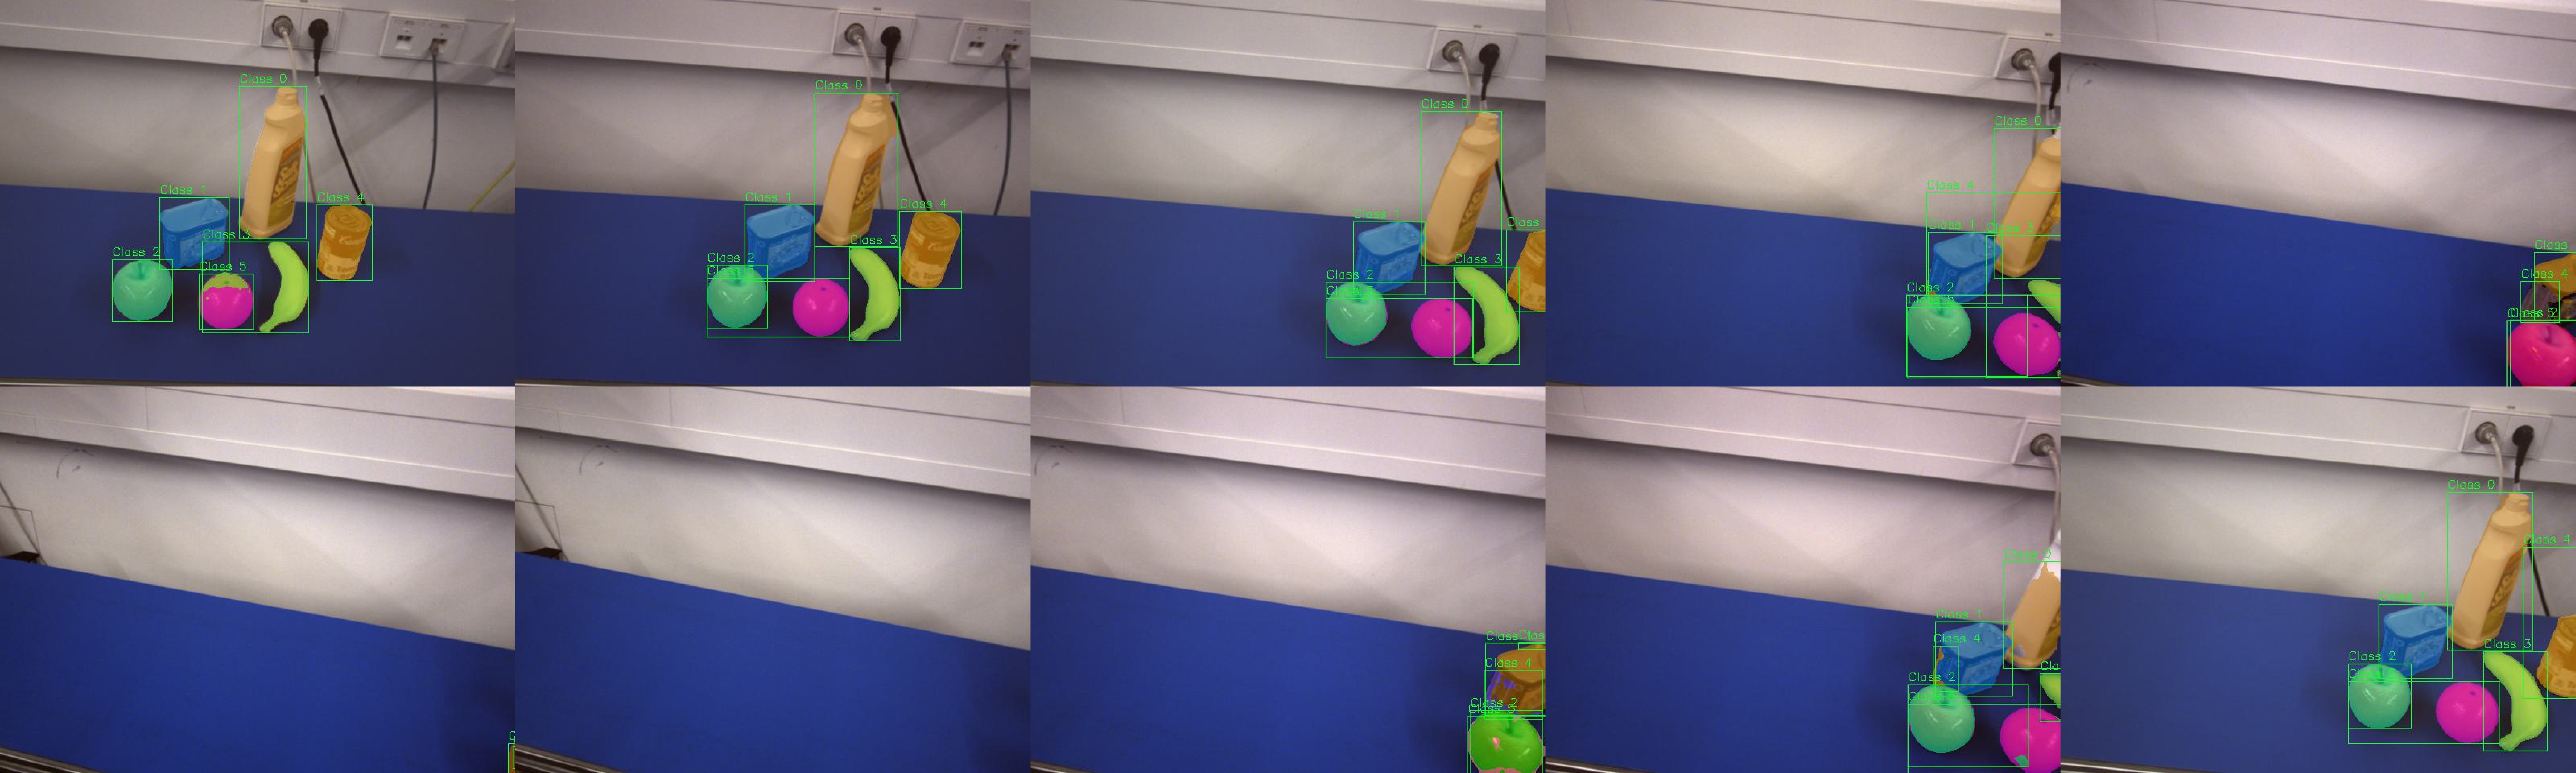
\includegraphics[width=1.\linewidth]{figures/qualitative_analysis_stereo/converer_belt_easy_overlays_onseg.pdf}
    }
    \caption{Inference on conveyor belt sequence 
    }
    \label{fig:qualitative_conveyor}
  \end{figure}